\documentclass[%
%oneside,                 % oneside: electronic viewing, twoside: printing
%$final,                   % draft: marks overfull hboxes, figures with paths
10pt]{article}

\listfiles               %  print all files needed to compile this document

\usepackage{relsize,makeidx,color,setspace,amsmath,amsfonts,amssymb}
\usepackage[table]{xcolor}
\usepackage{bm,ltablex,microtype}
\usepackage{graphicx}
\usepackage{sidecap}

\usepackage[T1]{fontenc}
%\usepackage[latin1]{inputenc}
\usepackage{ucs}
\usepackage[utf8x]{inputenc}

\usepackage{lmodern}

% Hyperlinks in PDF:
\definecolor{linkcolor}{rgb}{0,0,0.4}
\usepackage{hyperref}
\hypersetup{
    breaklinks=true,
    colorlinks=true,
    linkcolor=linkcolor,
    urlcolor=linkcolor,
    citecolor=black,
    filecolor=black,
    %filecolor=blue,
    pdfmenubar=true,
    pdftoolbar=true,
    bookmarksdepth=3   % Uncomment (and tweak) for PDF bookmarks with more levels than the TOC
    }
%\hyperbaseurl{}   % hyperlinks are relative to this root

% Tricks for having figures close to where they are defined:
% 1. define less restrictive rules for where to put figures
\setcounter{topnumber}{2}
\setcounter{bottomnumber}{2}
\setcounter{totalnumber}{4}
\renewcommand{\topfraction}{0.95}
\renewcommand{\bottomfraction}{0.95}
\renewcommand{\textfraction}{0}
\renewcommand{\floatpagefraction}{0.75}
% floatpagefraction must always be less than topfraction!
% 2. ensure all figures are flushed before next section
\usepackage[section]{placeins}
% 3. enable begin{figure}[H] (often leads to ugly pagebreaks)
%\usepackage{float}\restylefloat{figure}

\usepackage[framemethod=TikZ]{mdframed}


\setcounter{secnumdepth}{3}
\setcounter{tocdepth}{3}
\begin{document}

\thispagestyle{empty}

\begin{center}
{\LARGE\bf
\begin{spacing}{1.25}
Machine Learning and Artificial Intelligence activities at FRIB
\end{spacing}
}
\end{center}

\tableofcontents
\newpage

\section{Explanation}


The purpose of this document is to collect information about the  competence  in the area of ML/AI at FRIB Laboratory. This material is important to inform the upcoming events, e.g.,  \href{https://www.jlab.org/conference/AI2020}{\it AI for Nuclear Physics Workshop} at JLab, March 4-6, 2020; \href{https://conferences.lbl.gov/event/292/}{\it Workshop for Applied Nuclear Data Activities} at George Washington University, March 3-5, 2020;
and other related  activities.


\subsection{Description of individual entries}
Please format your entry (1 entry per page) according to the following template:

\vspace{5mm}
\noindent
\fbox{\begin{minipage}{0.98\linewidth}
{\bf Topic} (in subsubsection title. Capitalize words)
\begin{description}
\item[Participants] List local faculty/staff, research associates (p), students (g,u). External collaborators should be listed as co-authors in references.
\item[Description] Provide a short paragraph ($<$600 characters; think of a PRL abstract) describing the ML/AI aspects of the project. To provide uniformity, use the acronyms defined in Sec.~\ref{acronyms}
\item[FRIB relevance] ($<$600 characters) 
\item[Outcomes] List instrumentation outcomes, if any. Provide your published/submitted/anticipated papers with {\bf hyperlinks}. 
\end{description}
You are encouraged to provide a figure below the description. If needed, use  side captions as in entry~\ref{sidecaption}.
\end{minipage}}

\section{Machine Learning and AI in Nuclear Physics}


Artificial intelligence (AI)-based techniques, particularly in machine
learning (ML) and optimization, are increasingly being used in many areas
of experimental and theoretical physics to facilitate discovery,
accelerate data analysis and modeling efforts, and bridge different
physical and temporal scales in numerical models.
The large amount of degrees of freedom pertain to both theory and experiment in nuclear physics. With increasingly complicated experiments that produce large amounts data, automated classification of events becomes increasingly important. 
Artificial intelligence and Machine Learning   techniques are proving to be powerful tools for advancing our
understanding of the physics from complicated nuclear systems. 



\subsection{Types of Machine Learning}



The approaches to machine learning are many, but are often split into two main categories. 
In \emph{supervised learning} we have a situation with known input and output data that we want to reproduce with a given set of models, letting the given machine learning algorithm deduce the eventual logic behind our data. 

On the other hand, \emph{unsupervised learning}
is a method for finding patterns and relationship in data sets without any prior knowledge of the system.
Some authors also operate with a third category, namely \emph{reinforcement learning}. This is a paradigm 
of learning inspired by behavioural psychology, where learning is achieved by trial-and-error, 
solely from rewards and punishment.

Some of the most common tasks are:

\begin{itemize}
  \item Classification: Outputs are divided into two or more classes. The goal is to   produce a model that assigns inputs into one of these classes. An example is to identify  digits based on pictures of hand-written ones. 

  \item Regression: Finding a functional relationship between an input data set and a reference data set.   The goal is to construct a function that maps input data to continuous output values.

  \item Clustering: Data are divided into groups with certain common traits, without knowing the different groups beforehand.  It is thus a form of unsupervised learning.
\end{itemize}
These categories are all part of the broad spectrum of AI and ML techniques being studied at FRIB. 


\subsection{Acronyms of machine learning/statistical terms used}\label{acronyms}

We list here various acronyms used in the description of the different AI/ML projects.

\begin{description}
\item[AE] Auto encoders
\item[AI] Artificial intelligence
\item[ANN] Artificial neural networks
\item[BC] Bayesian calibration
\item[BM] Boltzmann machines
\item[BMA] Bayesian model averaging
\item[BML] Bayesian machine learning
\item[BNN] Bayesian neural networks
\item[BS] Bayesian statistics
\item[CI] Credibility interval
\item[CL] Clustering
\item[CNN] Convolutional neural networks
\item[CoD] Coefficient of determination
\item[DL] Deep learning
\item[DRB] Decision trees, random forests and boosting
\item[ECP] Empirical coverage probability
\item[FS] Frequentist statistics
\item[GM] Graphical models
\item[GP] Bayesian Gaussian processes
\item[LHC] Large Hadron Collider at CERN
\item[KR] Kernel regression
\item[LR] Logistic regression
\item[LSTM] Long short-term memory
\item[MCMC] Markov chain Monte Carlo
\item[ML] Machine learning
\item[NN] Neural networks
\item[PCA] Principal component analysis and dimensionality reduction techniques
\item[REG] Linear regression 
\item[RL] Reinforcement learning
\item[RNN] Recurrent neural networks
\item[RHIC] Relativistic Heavy Ion Collider at Brookhaven Natl. lLdk
\item[SL] Supervised learning
\item[SVM] Support vector machines
\item[UQ] Uncertainty quantification
\item[VAE] Variational auto encoders
\end{description}

\clearpage
\newpage

\section{AI/ML projects at FRIB}

\subsection{Accelerators/Beam Tuning}

%%%%%%%%%%%%%%%%%%%%%%  Entry Begins %%%%%%%%%%%%%%%%%%%%%%%%%
\subsubsection{Artificial Intelligence Aided Beam Tuning}
\vspace{5mm}
\noindent
\fbox{\begin{minipage}{0.96\linewidth}
\begin{description}
%%%
\item[Participants:] Y.Hao, S.Lidia, T.Maruta, L.Neufcourt(p), A.Plastun and T.Zhang
%%%
\item[Description:] The capability of providing versatile species of ions presents a challenge of fast accelerator tuning of the new ion species to maintain the high availability of scientific discoveries.  The recent progress on AI shines a light on a new approach to achieve fast tuning.  We propose to establish a data-refined accelerator model for fast tuning using AI based on the existing diagnostic data.  The proposed work including the inference of parameters in the accelerator model and creating a surrogate model using the GP or ANN for the components that cannot be well predicted by physics model.
%%%
\item[FRIB relevance:] The ML and BS application in Beam tuning provide new methods to quickly switch the operation modes of FRIB.
%%%
\item[References:] {\it Y. Hao and L. M. Neufcourt, “Application of Bayesian Inference in Accelerator Commissioning of FRIB”, in Proc. 10th Int. Particle Accelerator Conf. (IPAC'19), Melbourne, Australia, May 2019}

\end{description}
%%%
\end{minipage}
}
\begin{figure}[htb!]
%%%% for side caption use \begin{SCfigure}[10][b]... \end{SCfigure}
\centering
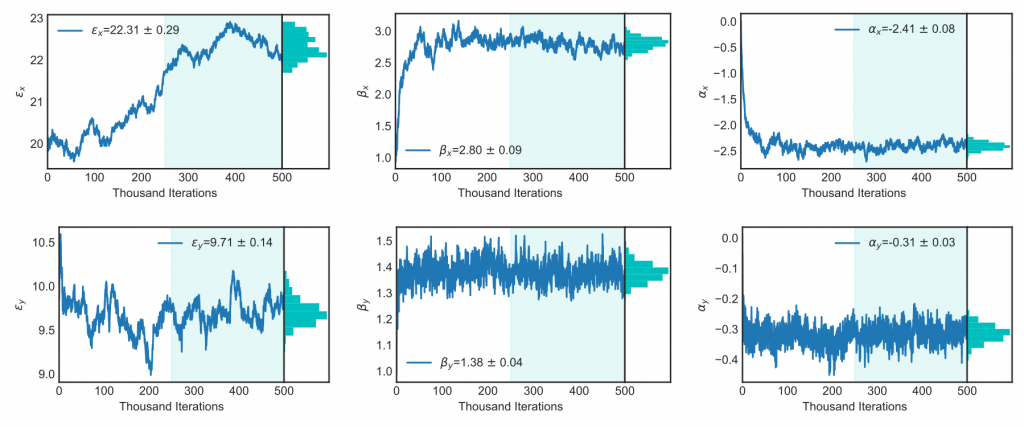
\includegraphics[width=\linewidth]{figures/bayesian_inference_FRIB.png}
\caption{The iterations of inferring the beam linear properties at the exit of the ion source using Bayesian Inference}
\end{figure}
\clearpage
\newpage
%%%%%%%%%%%%%%%%%%%%%%  Entry Ends %%%%%%%%%%%%%%%%%%%%%%%%%

%%%%%%%%%%%%%%%%%%%%%%  Entry Begins %%%%%%%%%%%%%%%%%%%%%%%%%
\subsubsection{Beam loss Control and Machine Protection with Artificial Intelligence}
\vspace{5mm}
\noindent
\fbox{\begin{minipage}{0.96\linewidth}
\begin{description}
%%%
\item[Participants:] Y.Hao, S.Lidia, L.Neufcourt(p) and T.Zhang
%%%
\item[Description:] The beam loss control and high-fidelity machine protection system are essential tasks to achieve the 400 KW ion beam power in FRIB.  Artificial intelligence provides a powerful toolset in predicting and localizing the beam loss, anomaly detection and unloading the risk of the hardware damage due to beam loss.   We propose to create a surrogate model with GP or ANN to identify the correlation of beam properties and the beam loss using diagnostic data from BPMs and loss monitors, ‘forecast’ and prevent the hardware damage due to excess power from beam loss.
%%%
\item[FRIB relevance:] The surrogate model create by AI may largely protect the accelerator from damaging or degrading due to beam losses and improve the availability of the accelerator.
%%%
\item[References:] {\it None}

\end{description}
%%%
\end{minipage}
}

\clearpage
\newpage
%%%%%%%%%%%%%%%%%%%%%%  Entry Ends %%%%%%%%%%%%%%%%%%%%%%%%%
%%%%%%%%%%%%%%%%%%%%%%  Entry Begins %%%%%%%%%%%%%%%%%%%%%%%%%
\subsubsection{Machine learning SECAR tuning optimization}\label{sidecaption}
\vspace{5mm}
\noindent
\fbox{\begin{minipage}{0.98\linewidth}
\begin{description}
\item[Participants] F. Montes, H. Schatz,  K. Hermansen (g), S. Ayoub (g), D. Crisp, T. Summers and A.M. Amthor (Bucknell)
\item[Description] The primary purpose of the The SEparator for CApture Reactions (SECAR) at FRIB is to measure resonance strengths in radiative proton and alpha capture reactions for astrophysics. We have developed and tested systems to interpret data in real-time from existing spectrometer and beam-line systems to tune multiple elements to provide desired beam properties without providing the autonomous system a theoretical model of the particle-optical system being tuned. 
%This autonomous beam tuning was the first technique to produce nearly 100\% transmission through the target aperture in the SECAR target system. 
Preliminary SECAR optimization simulations have shown that such a technique can also be used to produce an achromatic dispersive image in SECAR by using autonomous optimization approaches such as a GP, NN and/or the Particle Swarm method. We are now working toward a further test of the automated optimization to 
%correctly tune the incoming beam into SECAR and to <We already did this, no?>
independently minimize the beam-spot size at different critical positions in SECAR, thus maximizing beam purity and mass resolving power, which are critical to maximizing the scientific productivity of SECAR. 
\item[FRIB relevance] Automated optimization is expected to reduce tuning time and improve quality and consistency of SECAR performance. These techniques are also applicable to other FRIB accelerator, beam-line, and spectrometer systems. 
\item[References:] {\it Experimental test of an online ion-optics optimizer,  Amthor A.~M., Schillaci Z.~M., Morrissey D.~J., Portillo M., Schwarz S., Steiner M., Sumithrarachchi C.}
\href{https://ui.adsabs.harvard.edu/link_gateway/2018NIMPA.895...90A/doi:10.1016/j.nima.2018.04.001}{Nuc. Inst. and Meth. in Phys. Res. A, 895, 90 (2018)}
\end{description}
\end{minipage}}

\begin{SCfigure}[1][b]
\centering
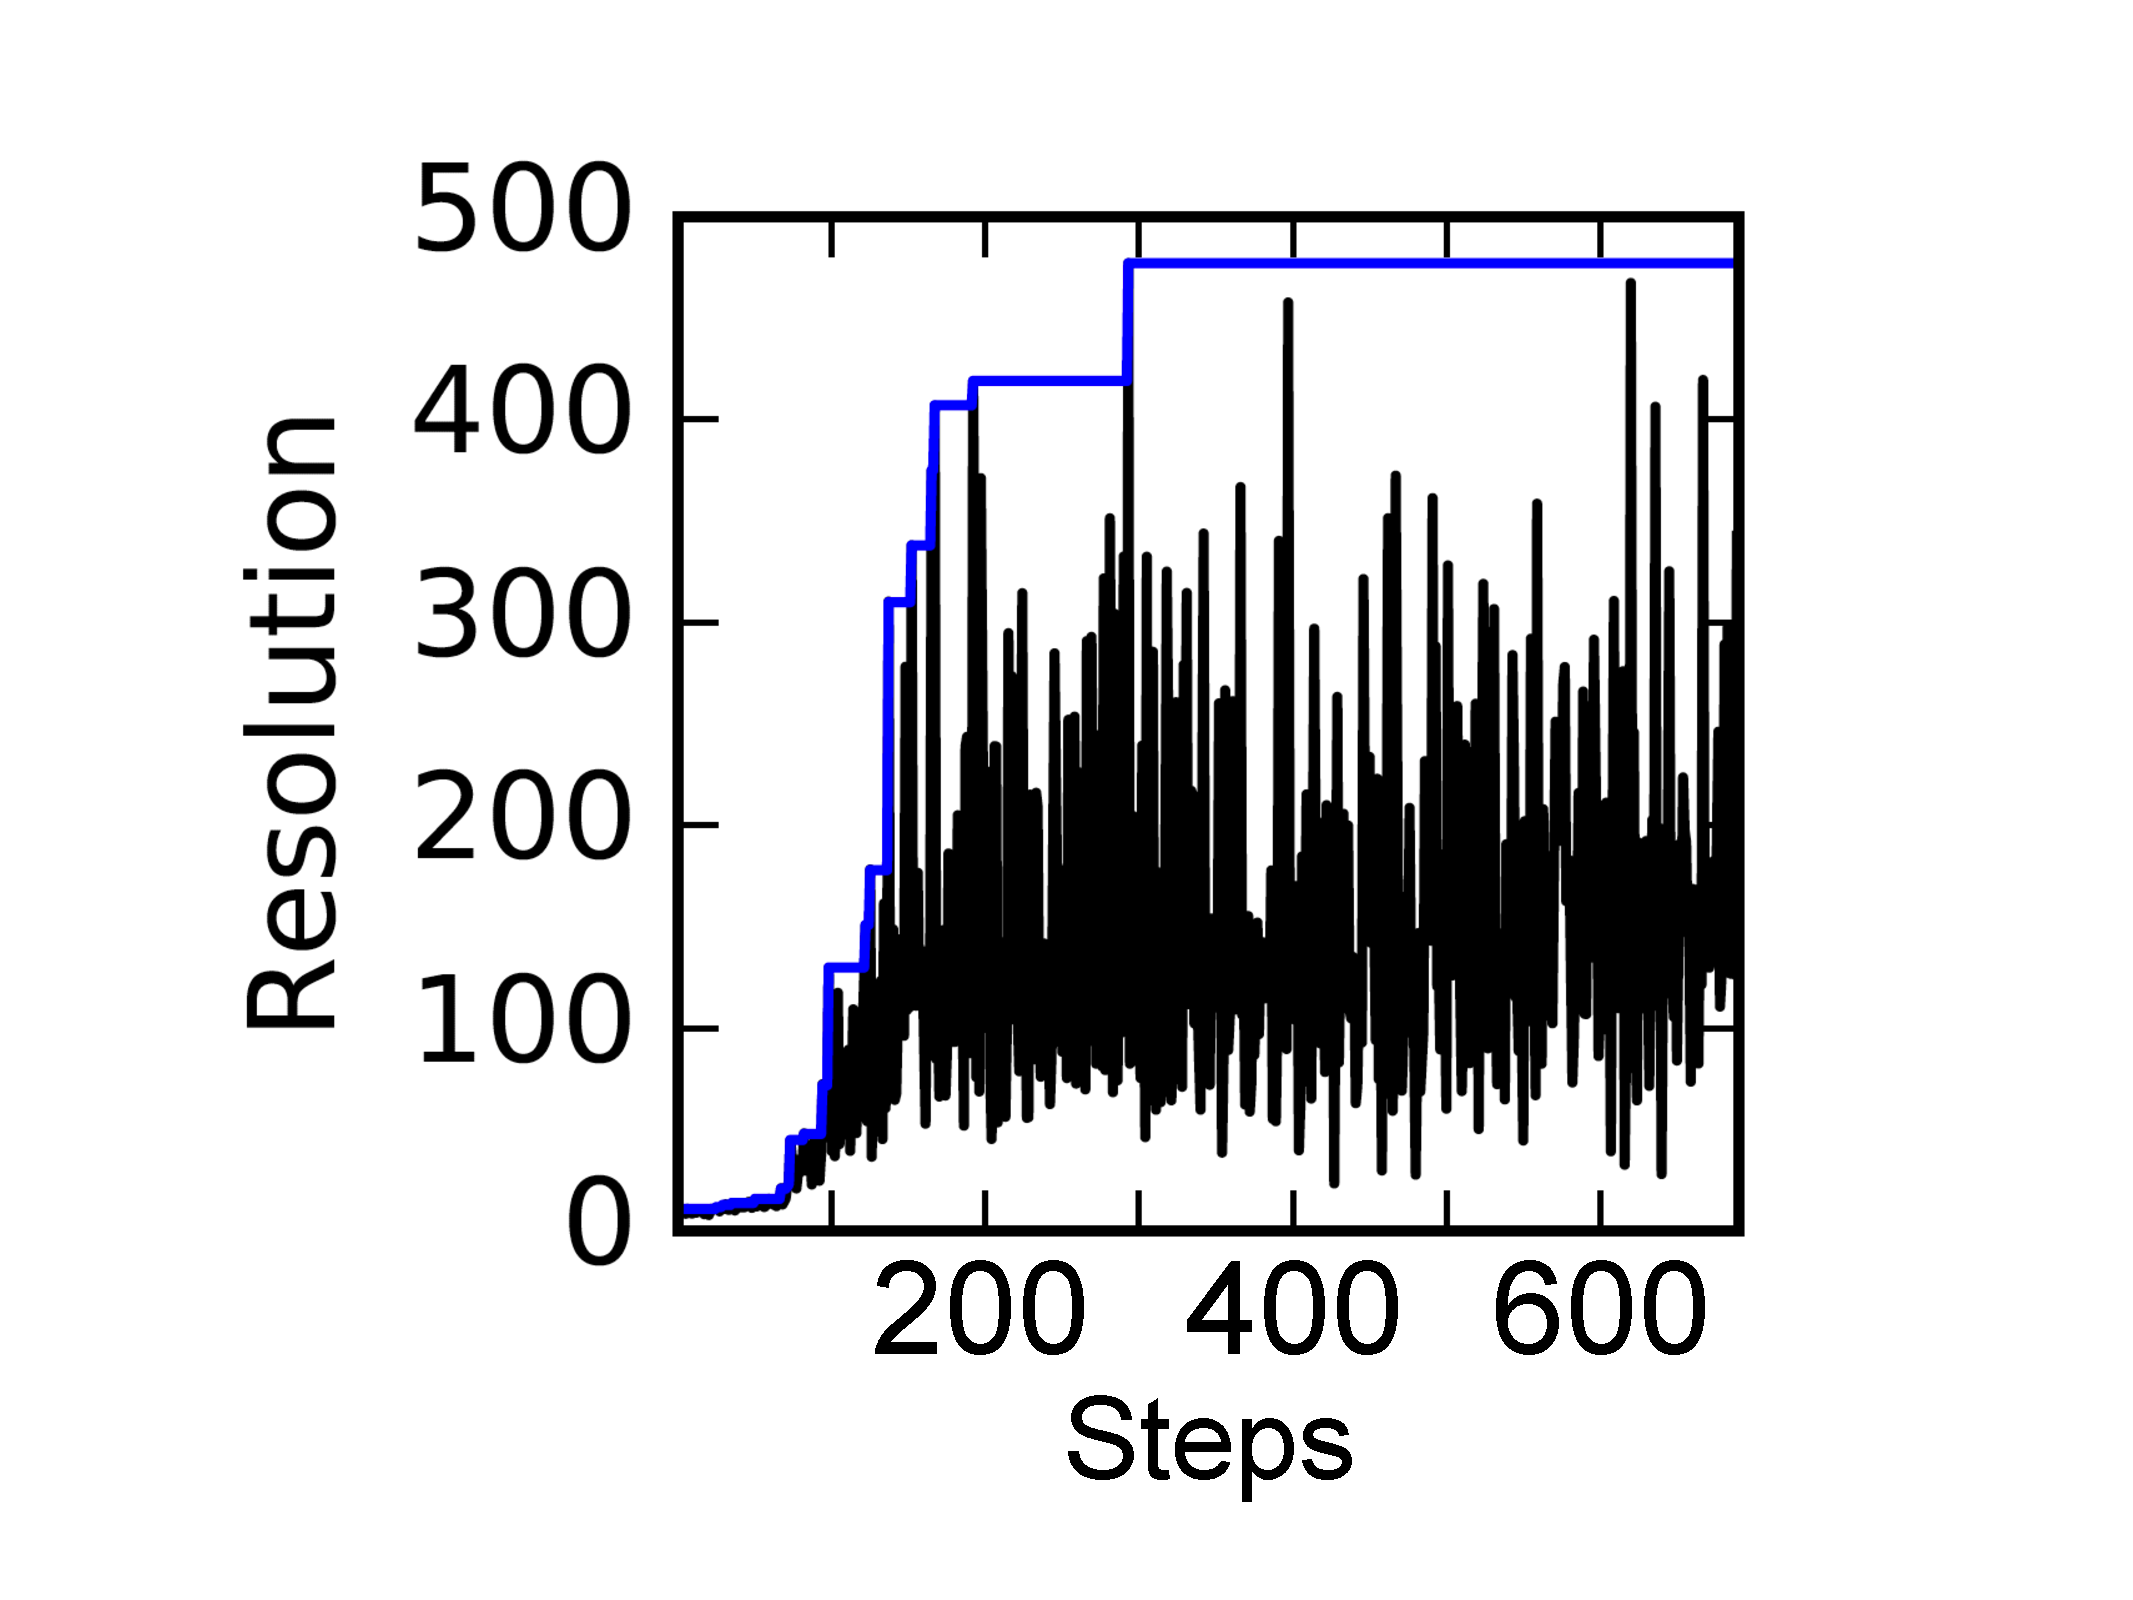
\includegraphics[width=0.55\linewidth]{figures/SECAR_optimization.pdf}
\caption{SECAR mass resolution as a function of the number steps in the optimization. Each step corresponds to a different optics configuration.}
\end{SCfigure}

\clearpage
\newpage
%%%%%%%%%%%%%%%%%%%%%%  Entry Ends %%%%%%%%%%%%%%%%%%%%%%%%%




\subsection{Detectors}
\subsubsection{Gamma-ray Tracking}
\vspace{5mm}
\noindent
\fbox{\begin{minipage}{0.96\linewidth}
\begin{description}
%%%
\item[Participants:] D. Weisshaar, A. Gade, L. Neufcourt, J. Chung
\item[Description:]  Gamma-ray tracking algorithms determine how many $\gamma$ rays got fully or partially absorbed in an event by analyzing the measured interaction positions and energy depositions. 
%%ML techniques like NN are trained on measured data sets by analyzing the pattern of interaction points. 
Experimental energy measurements and computer simulations can constitute a large set of data
on which ML models such as neural networks can be trained to identify patterns in interaction points.
This approach does make no assumption about the underlying scattering processes (Compton scatter, Photo effect, pair production) as state-of-the-art deterministic algorithms do, especially the handling of wrongly reported interaction points by the detectors. 

%%%
\item[FRIB relevance:] The Gamma-Ray Energy Tracking Array GRETA will be one of the premium devices at FRIB. Improvement on its tracking capability in terms of better identification of incomplete absorbed $\gamma$ rays will directly translate into better spectral quality and sensitivity of this device, enlarging its scientific reach. 
%%%
\item[References:] {none} 
\end{description}
%%%
\end{minipage}
}
\begin{figure}[htb!]
\centering
\caption{To be added}
\end{figure}
\clearpage
\newpage


\subsection{Data Analysis and Statistical Analysis}

\subsubsection{Machine learning methods for track classification in the AT-TPC}

\vspace{5mm}
\noindent
\fbox{\begin{minipage}{0.96\linewidth}
\begin{description}
%%%
\item[Participants:] D. Bazin, M. Hjorth-Jensen
%%%
\item[Description:] We have implemented several  ML methods for event classification in the Active-Target Time Projection Chamber (AT-TPC) detector at NSCL. In particular we have implemented advanced convolutional AE NN to the analysis of two-dimensional projections of particle tracks
from a resonant proton scattering experiment on $^{46}$Ar.


%%%
\item[FRIB relevance:] We expect that many of the new FRIB experiments will produce large amounts of data. A class of detectors such as the AT-TPC is able to detect several reaction channels simultaneously. Extracting low cross section channels requires to classify the events of interest, which requires a large degree of automation. We expect that these techniques will play a central role at FRIB. 
%%%
\item[References:] {\it Machine learning methods for track classification in the AT-TPC},  M.P.Kuchera, R.Ramanujan, J.Z.Taylor, R.R.Strauss, D.Bazin, J.Bradt, R.M. Chen,
\href{https://doi.org/10.1016/j.nima.2019.05.097}{Nucl. Inst. Meth. A 940, 56 (2019)}
\end{description}
%%%
\end{minipage}
}
\begin{figure}[htb!]
\centering
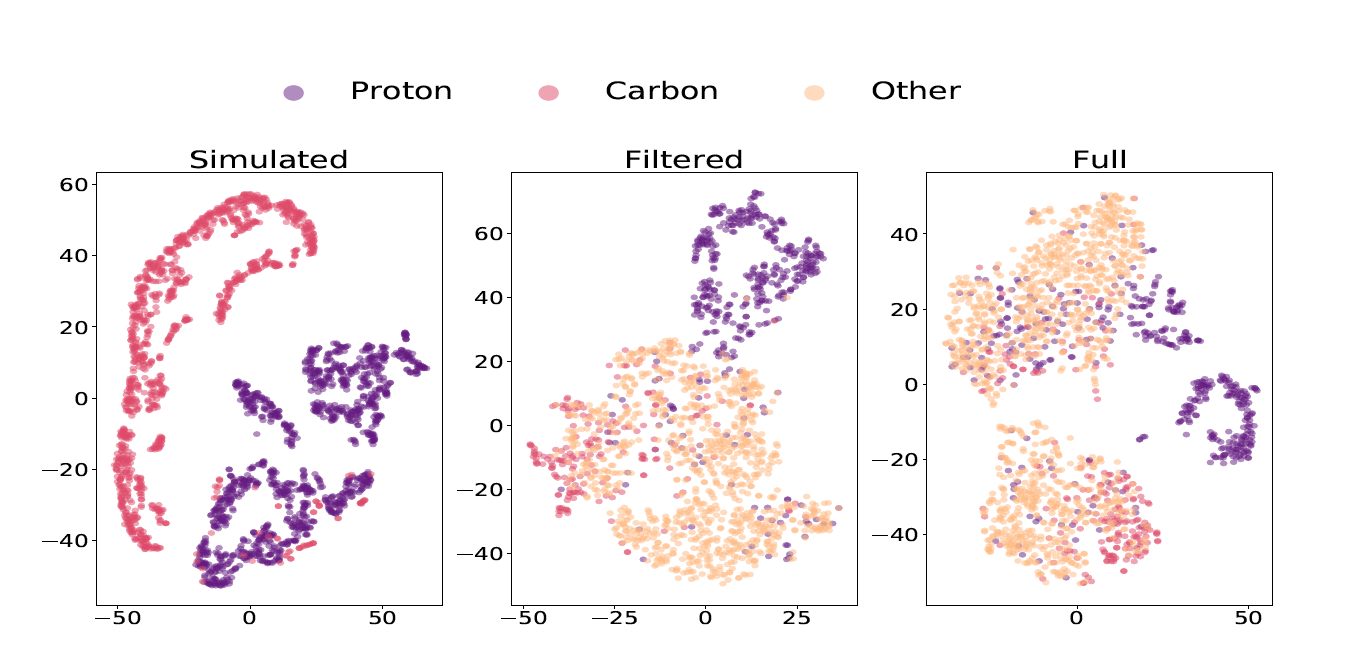
\includegraphics[width=\linewidth]{figures/attpc.png}
\caption{Visualization of the latent space from the VGG16 model on
three different data-sets.  The
axes have arbitrary non-informative units.}
\end{figure}
\clearpage
\newpage

\subsubsection{Machine learning for beta-decay experiments }

\vspace{5mm}
\noindent
\fbox{\begin{minipage}{0.96\linewidth}
\begin{description}
%%%
\item[Participants:] C. Dembsky (u), G. T. Ulvik (g), S. Liddick, M. Hjorth-Jensen
%%%
\item[Description:] When a neutron-rich
nucleus beta decays, a neutron transforms into a proton and emits an electron $\beta$. The excited nucleus can then interact electromagnetically with the surrounding orbital electrons. This can result in the ejection of an internal conversion electron $e^{-}$ from the atom.
Because this process is essentially simultaneous in time, it is pivotal to differentiate between the electron $\beta$ emitted from the nucleus and the internal conversion electron $e^{-}$ emitted from the atom. We have used, with success, various classification methods, in particular CNNs, AEs, RNNSs and VAEs to 
to distinguish between one and two electron events and predict the
electron(s) corresponding initial position(s).

%%%
\item[FRIB relevance:] We expect that many of the new FRIB experiments will produce large amounts of data. We expect that these techniques will play a central role at FRIB. 
%%%
\item[References:] 
\end{description}
%%%
\end{minipage}
}
\begin{figure}[htb!]
\centering
%\includegraphics[width=\linewidth]{figures/}
\caption{To be added
}
\end{figure}
\clearpage
\newpage



\subsubsection{Particle identifications in radiation detectors}
\vspace{5mm}
\noindent
\fbox{\begin{minipage}{0.98\linewidth}
\begin{description}
%%%
\item[Participants:] T. Ladourceur (u), C.Y. Tsang (g),  W.G. Lynch, M.B. Tsang
%%%
\item[Description:] In nuclear collisions, physics information is obtained from emitted charged particles measured with radiation detectors.  Identification of the emitted particles (PID) can be obtained from plotting the energy loss vs. total energy or momentum) as shown in the left panel of the figure. The data was obtained from S$\pi$RIT Time Projection Chamber. We test the ML algorithm using Monte Carlo events (right panel) from the TPC. A fully connected, feedforward NN classifier is used to separate out the various reaction products from simulated S$\pi$RIT data. Initially, we achieved an accuracy of $88\%$. However, with background tuning, we now achieve $97\%$, $92\%$, $85\%$, $77\%$ and $88\%$ for $\pi$, p, d, t, $^3$He and $\alpha$ particles respectively. We plan to train and tune the algorithm with real data. We will extend the method to identify the PID lines constructed from data taken with the NSCL High Resolution Array (HiRA). 
%%%
\item[FRIB relevance:] PID lines are ubiquitous observable in nearly all nuclear physics experiments that detect charged particles. ML tools and strategies will be needed for fast particle identifications to facilitate the huge amount of data from FRIB experiments.
%%%
\item[References:] {\it Non-linearity effects on the light-output calibration of light charged particles in CsI(Tl) scintillator crystals}, D. Dell'Aquila, S. Sweany,   et al., \href{https://doi.org/10.1016/j.nima.2019.03.065}{Nucl. Instrum. Methods Phys. Res. A 929 (2019) 162-172}.
%%%
\end{description}
%%%
\end{minipage}
}

\begin{figure}[htb!]
\centering
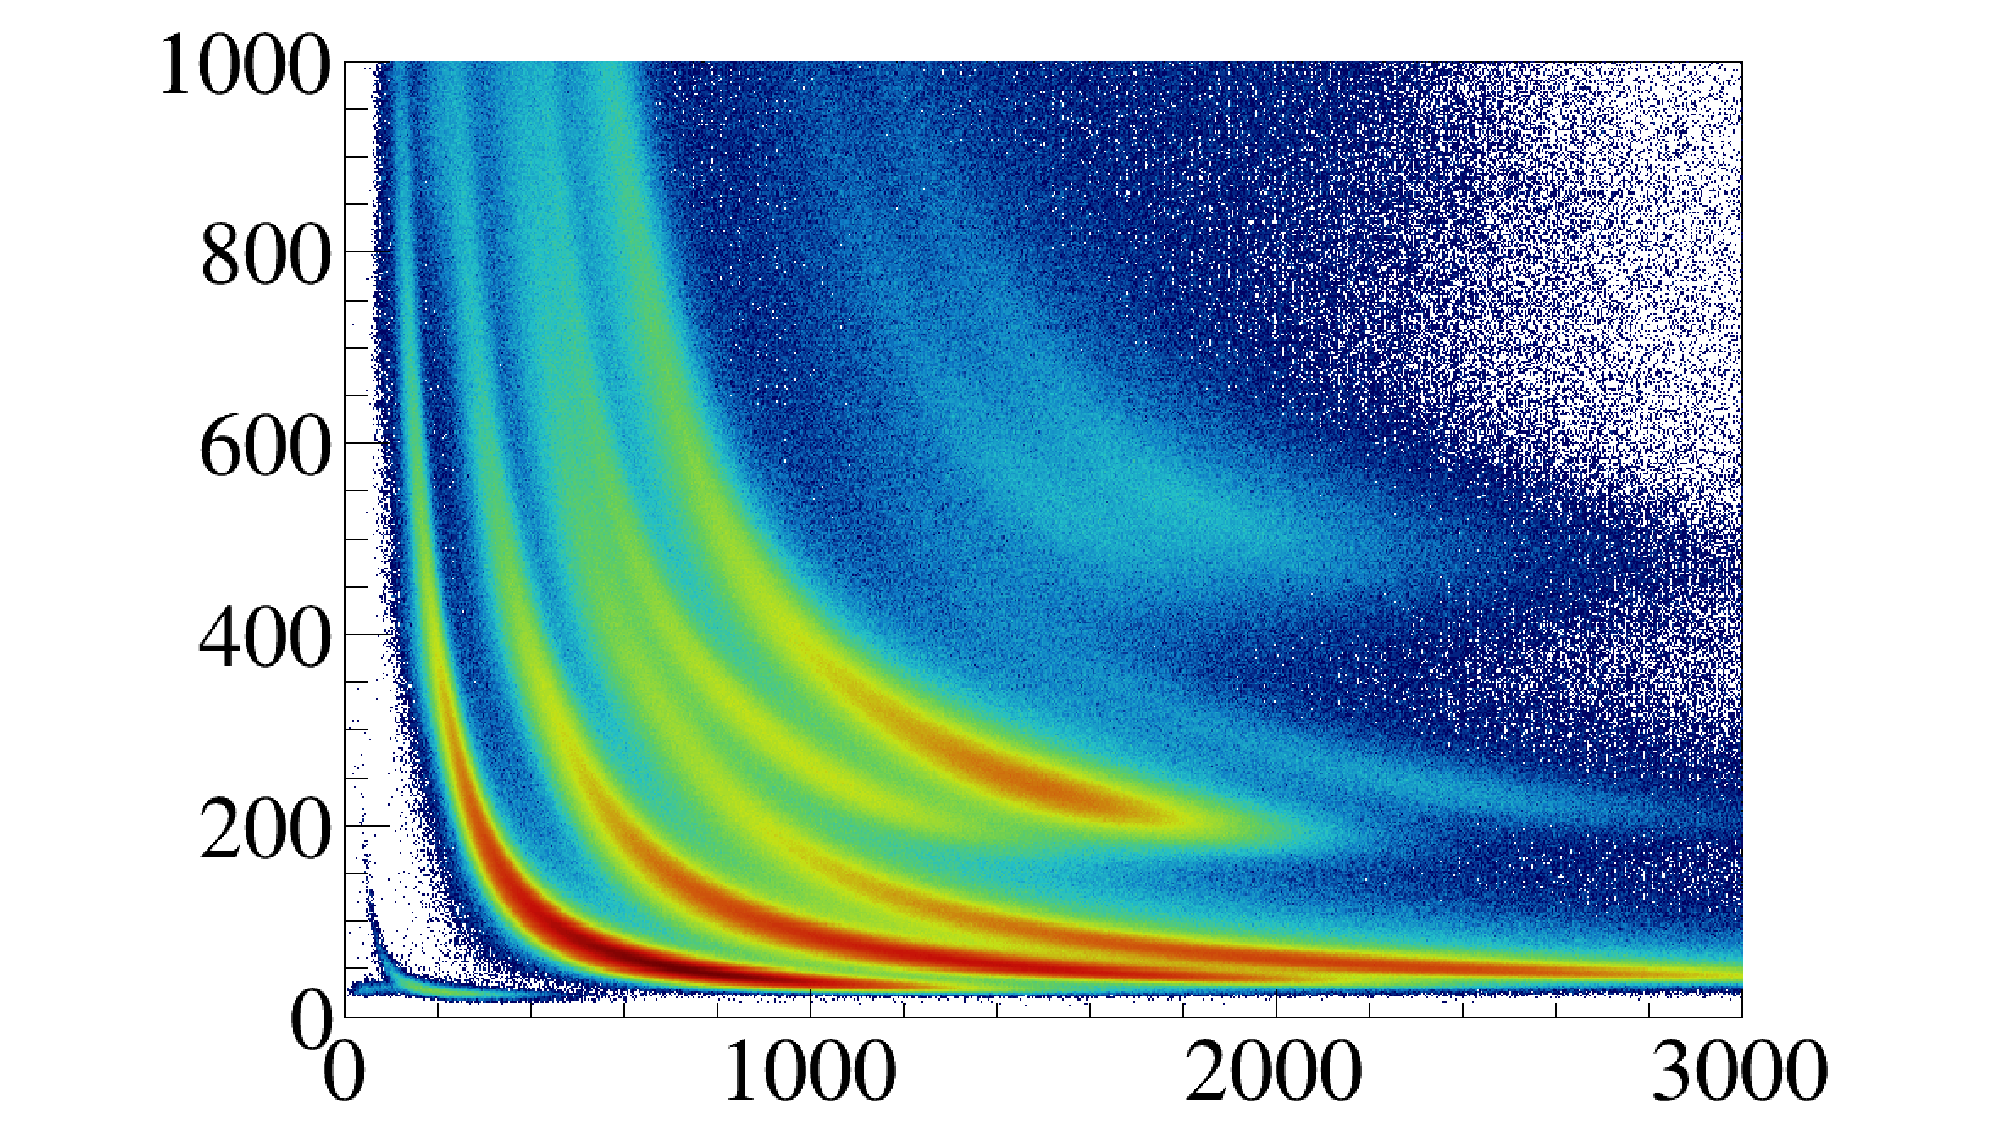
\includegraphics[width=0.49\linewidth]{figures/pid_sTPC_data.pdf}
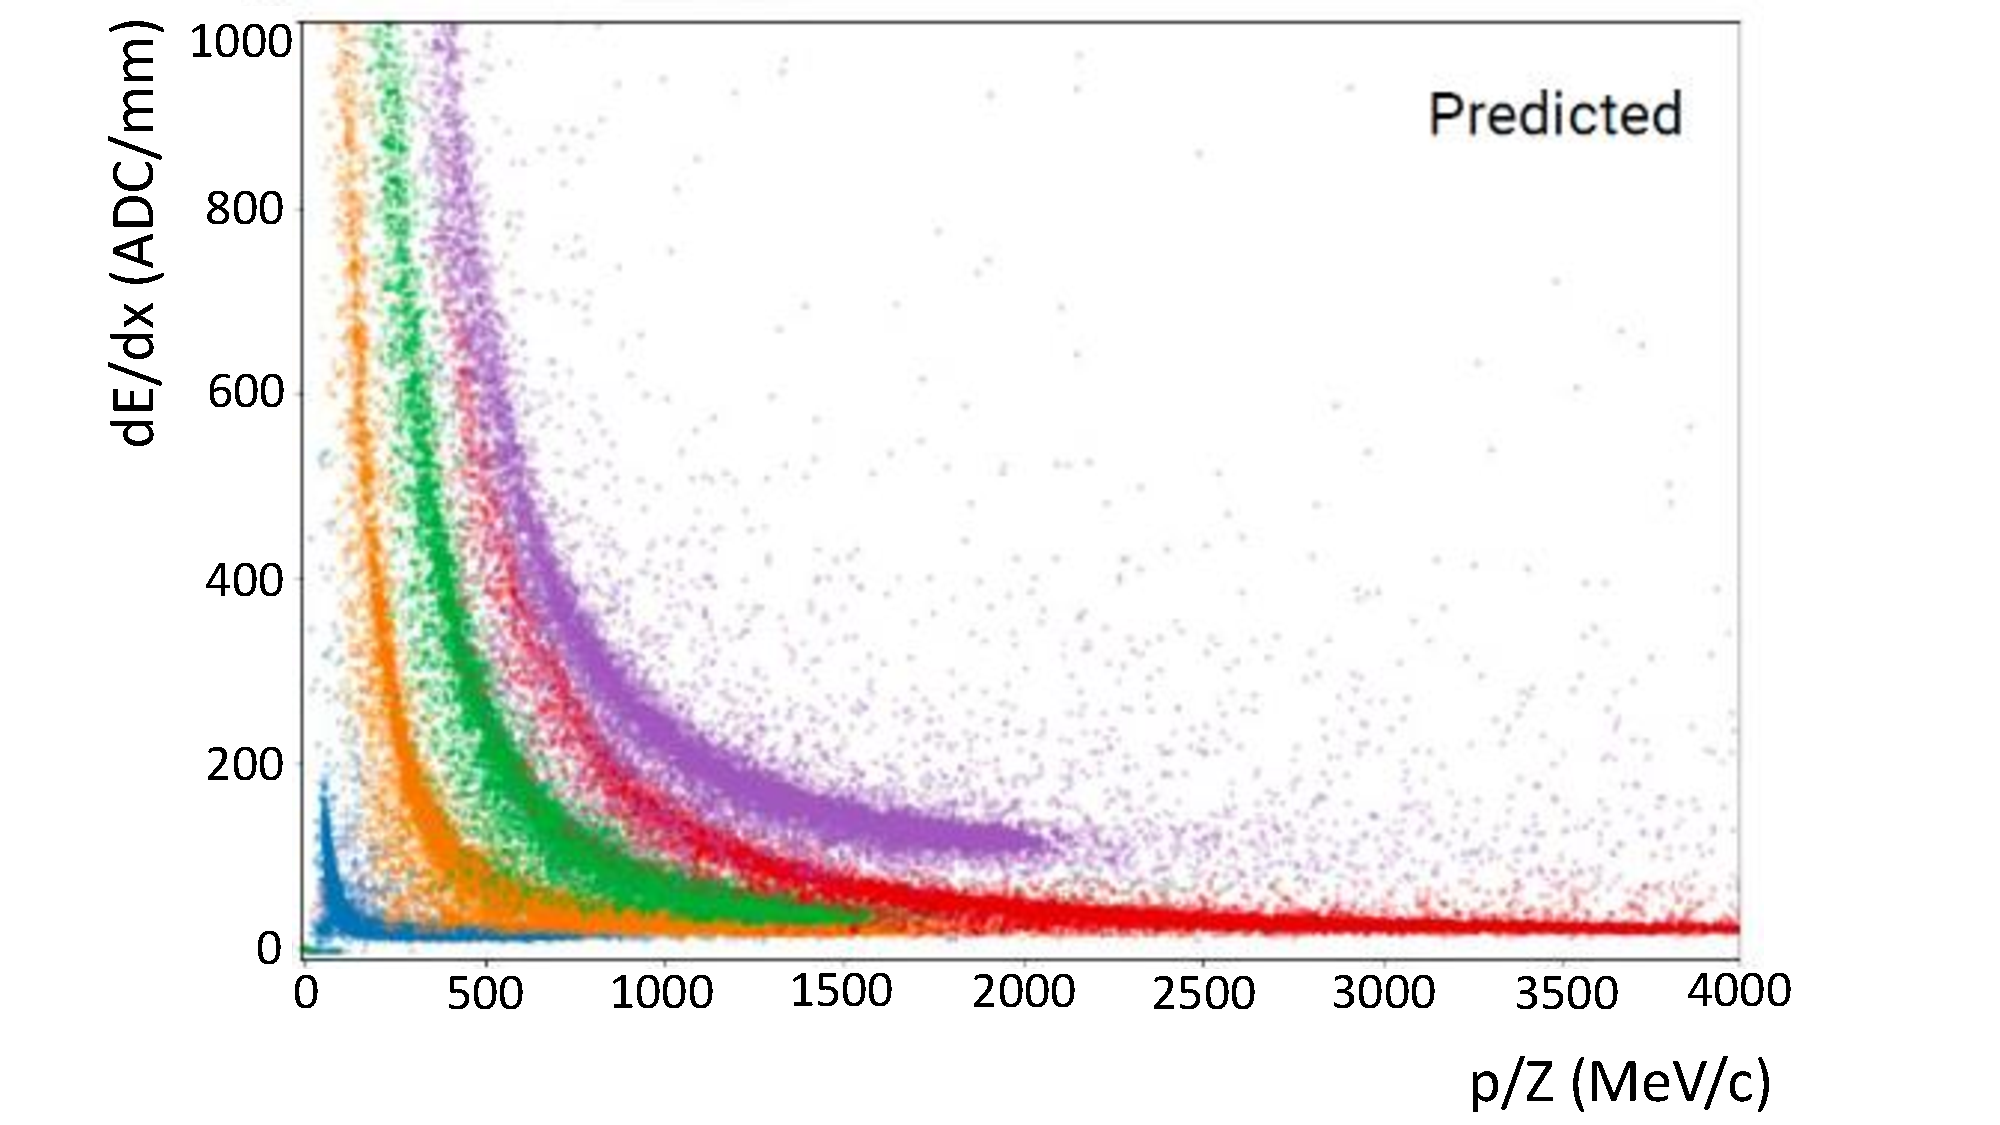
\includegraphics[width=0.49\linewidth]{figures/pid_sTPC_monte_carlo.pdf}
\caption{
(left panel) Particle identifications from $^{132}$Sn+$^{124}$Sn collisions at 270 MeV/u measured with the S$\pi$RIT TPC. (Right panel). Particle identifications from Monte Carlo events using Machine learning for $\pi^+$, p, d, t, $^3$He.
}
\end{figure}
\clearpage
\newpage


\subsection{Basic Research}

\subsubsection{Bayesian Approach to Extrapolations of Nuclear Observables}
\vspace{5mm}
\noindent
\fbox{\begin{minipage}{\linewidth}
\begin{description}
%%%
\item[Participants:] L. Neufcourt (p), Y. Cao (s), W. Nazarewicz, and F. Viens (STT)
%%%
\item[Description:]  To improve the quality of model-based predictions of nuclear properties of rare isotopes far from stability, we consider the information contained in the residuals in the regions where the experimental information exist.  The emulators of  residuals and CIs defining theoretical error bars are constructed using  GP  and BNN.
%%%
\item[FRIB relevance:] The proposed Bayesian SL approach to extrapolation of nuclear model predictions can be useful for assessing the impact of current and future FRIB experiments. The new capability to evaluate residuals is also expected to impact research in the domains where experiments are currently impossible, for instance, in simulations of the astrophysical $r$ process.
%%%
\item[References:] {\it Bayesian approach to model-based extrapolation of nuclear observables}, L. Neufcourt, Y. Cao, W. Nazarewicz, and F. Viens, \href{https://journals.aps.org/prc/abstract/10.1103/PhysRevC.98.034318}{Phys. Rev. C 98, 034318 (2018)} (Editor's Suggestion).
\end{description}
%%%
\end{minipage}
}
\begin{figure}[htb!]
\centering
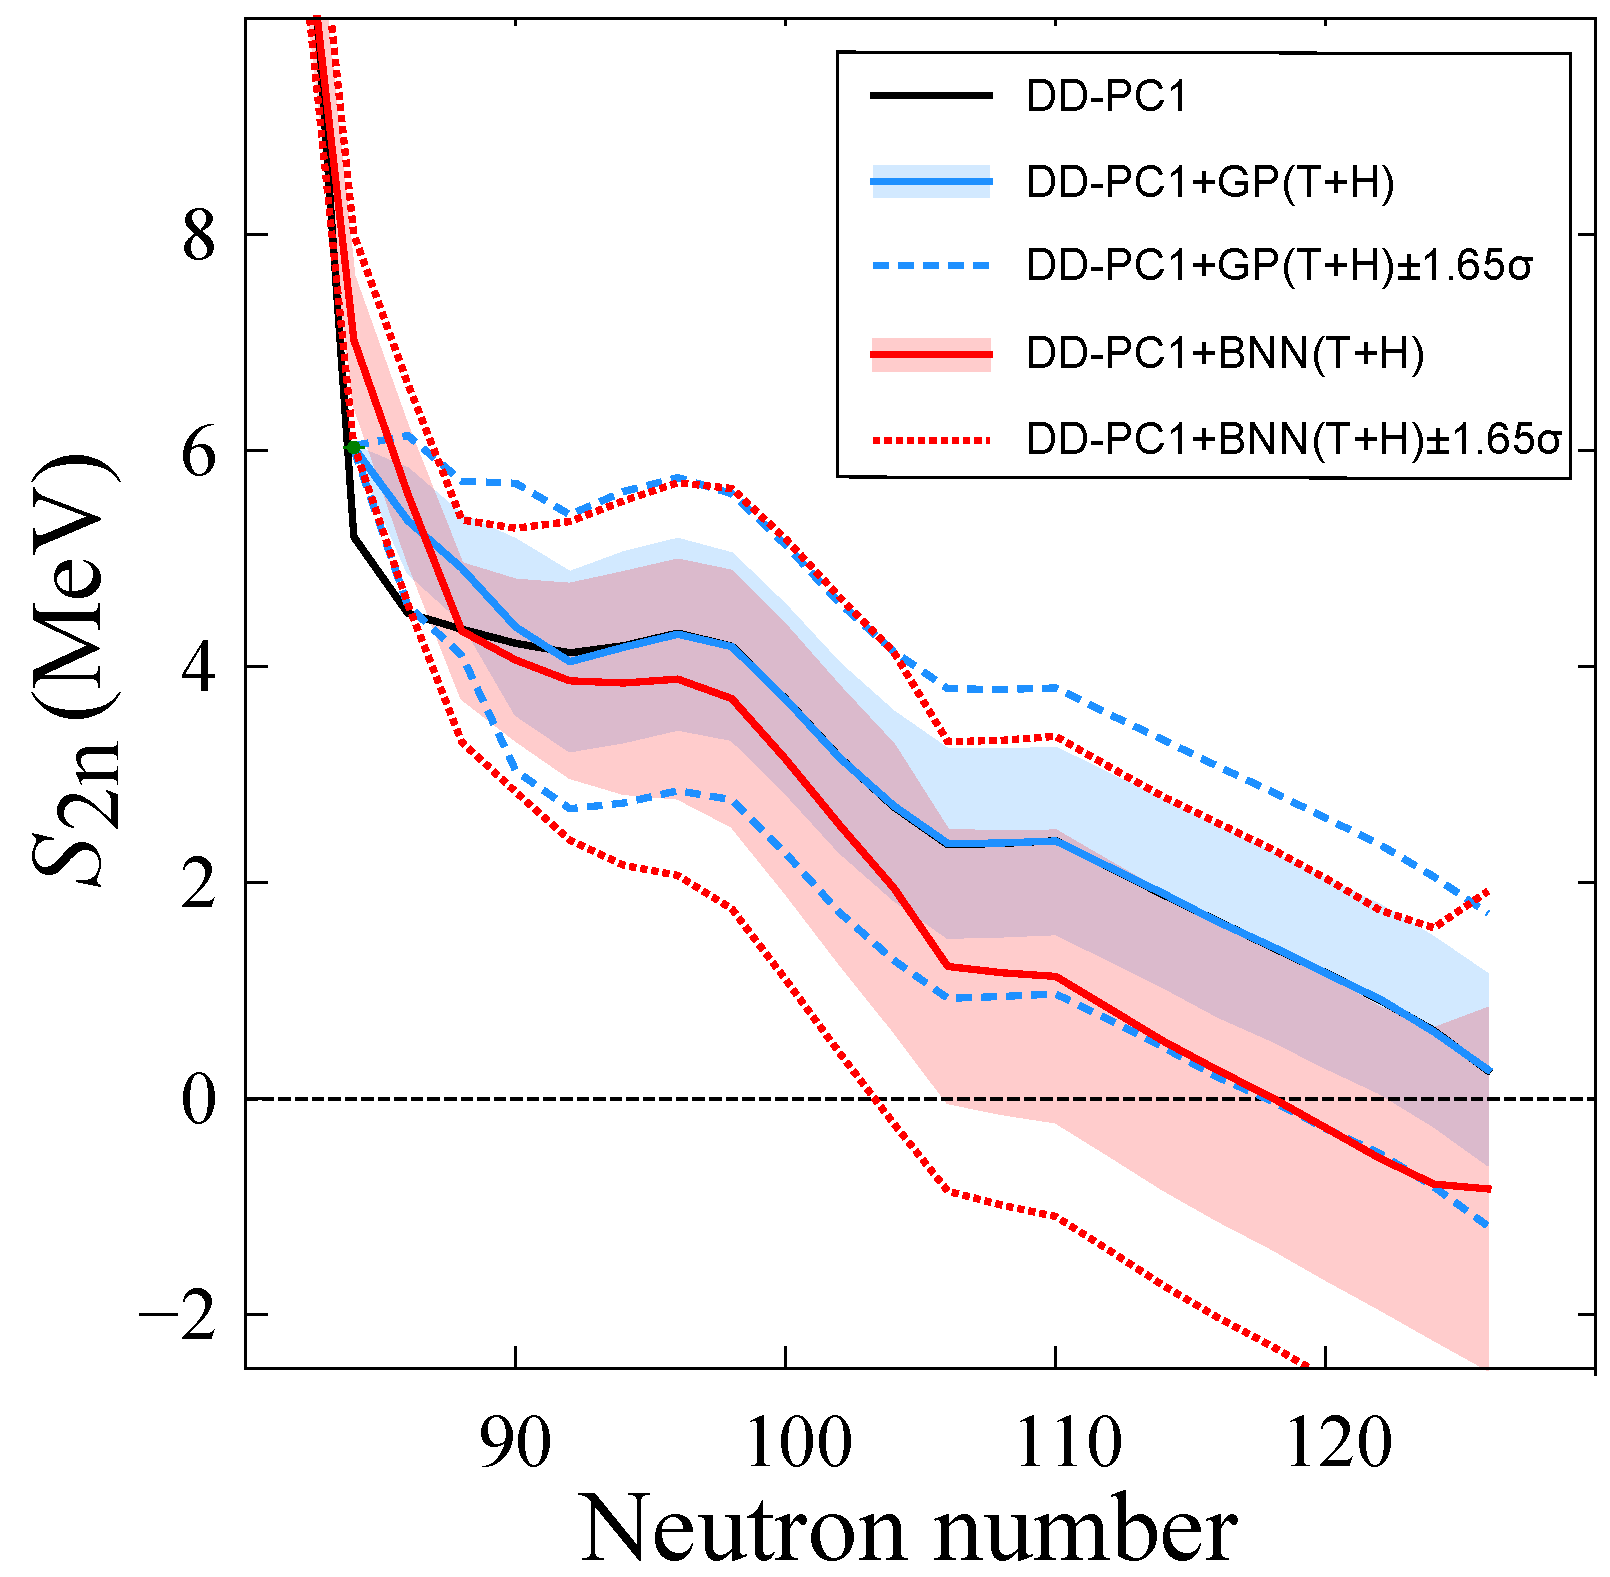
\includegraphics[width=0.63\linewidth]{figures/Sn-sep.pdf}
\caption{
Extrapolations of two-neutron separation energies for the even-even Sn chain
calculated  with DD-PC1 model  with statistical GP and BNN approaches.
One-sigma and 1.65-sigma CIs are marked.
}
\end{figure}


\clearpage

\newpage
\subsubsection{Nuclear Landscape with Bayesian Model Averaging}
\vspace{5mm}
\noindent
\fbox{\begin{minipage}{0.96\linewidth}
\begin{description}
%%%
\item[Participants:] L. Neufcourt (p), Y. Cao (g), S.A. Giuliani (p), W. Nazarewicz, F. Viens (STT), and O.B. Tarasov
%%%
\item[Description:] We use microscopic nuclear global mass models and Bayesian SL methodology to provide quantified predictions of proton and neutron separation energies  as well as Bayesian probabilities of existence
 throughout the nuclear landscape all the way to the particle drip lines. To account for uncertainties, Bayesian GP are trained on the separation-energy residuals for each individual model, and the resulting  predictions are  combined via BMA. This framework allows to account for systematic and statistical uncertainties and propagate them to extrapolative predictions. 
%%%
\item[FRIB relevance:] Considering the anticipated  FRIB production rates and uncertainties of theoretical predictions, we identified  regions, reached by FRIB, that are crucial for constraining theoretical mass models.
%%%
\item[References:] {\it Neutron Drip Line in the Ca Region from Bayesian Model Averaging}, \href{https://journals.aps.org/prl/abstract/10.1103/PhysRevLett.122.062502}{Phys. Rev. Lett. 122, 062502 (2019)};
{\it Beyond the proton drip line: Bayesian analysis of proton-emitting nuclei}, \href{https://journals.aps.org/prc/abstract/10.1103/PhysRevC.101.014319}{Phys. Rev. C 101, 014319 (2020)}; {\it Quantified limits of the nuclear landscape}, \href{https://arxiv.org/abs/2001.05924}{arXiv:2001.05924, submitted}.  L. Neufcourt, Y. Cao, S. Giuliani, W. Nazarewicz,  E. Olsen, F. Viens,and O.B. Tarasov
\end{description}
%%%
\end{minipage}
}
\begin{figure}[htb!]
\centering
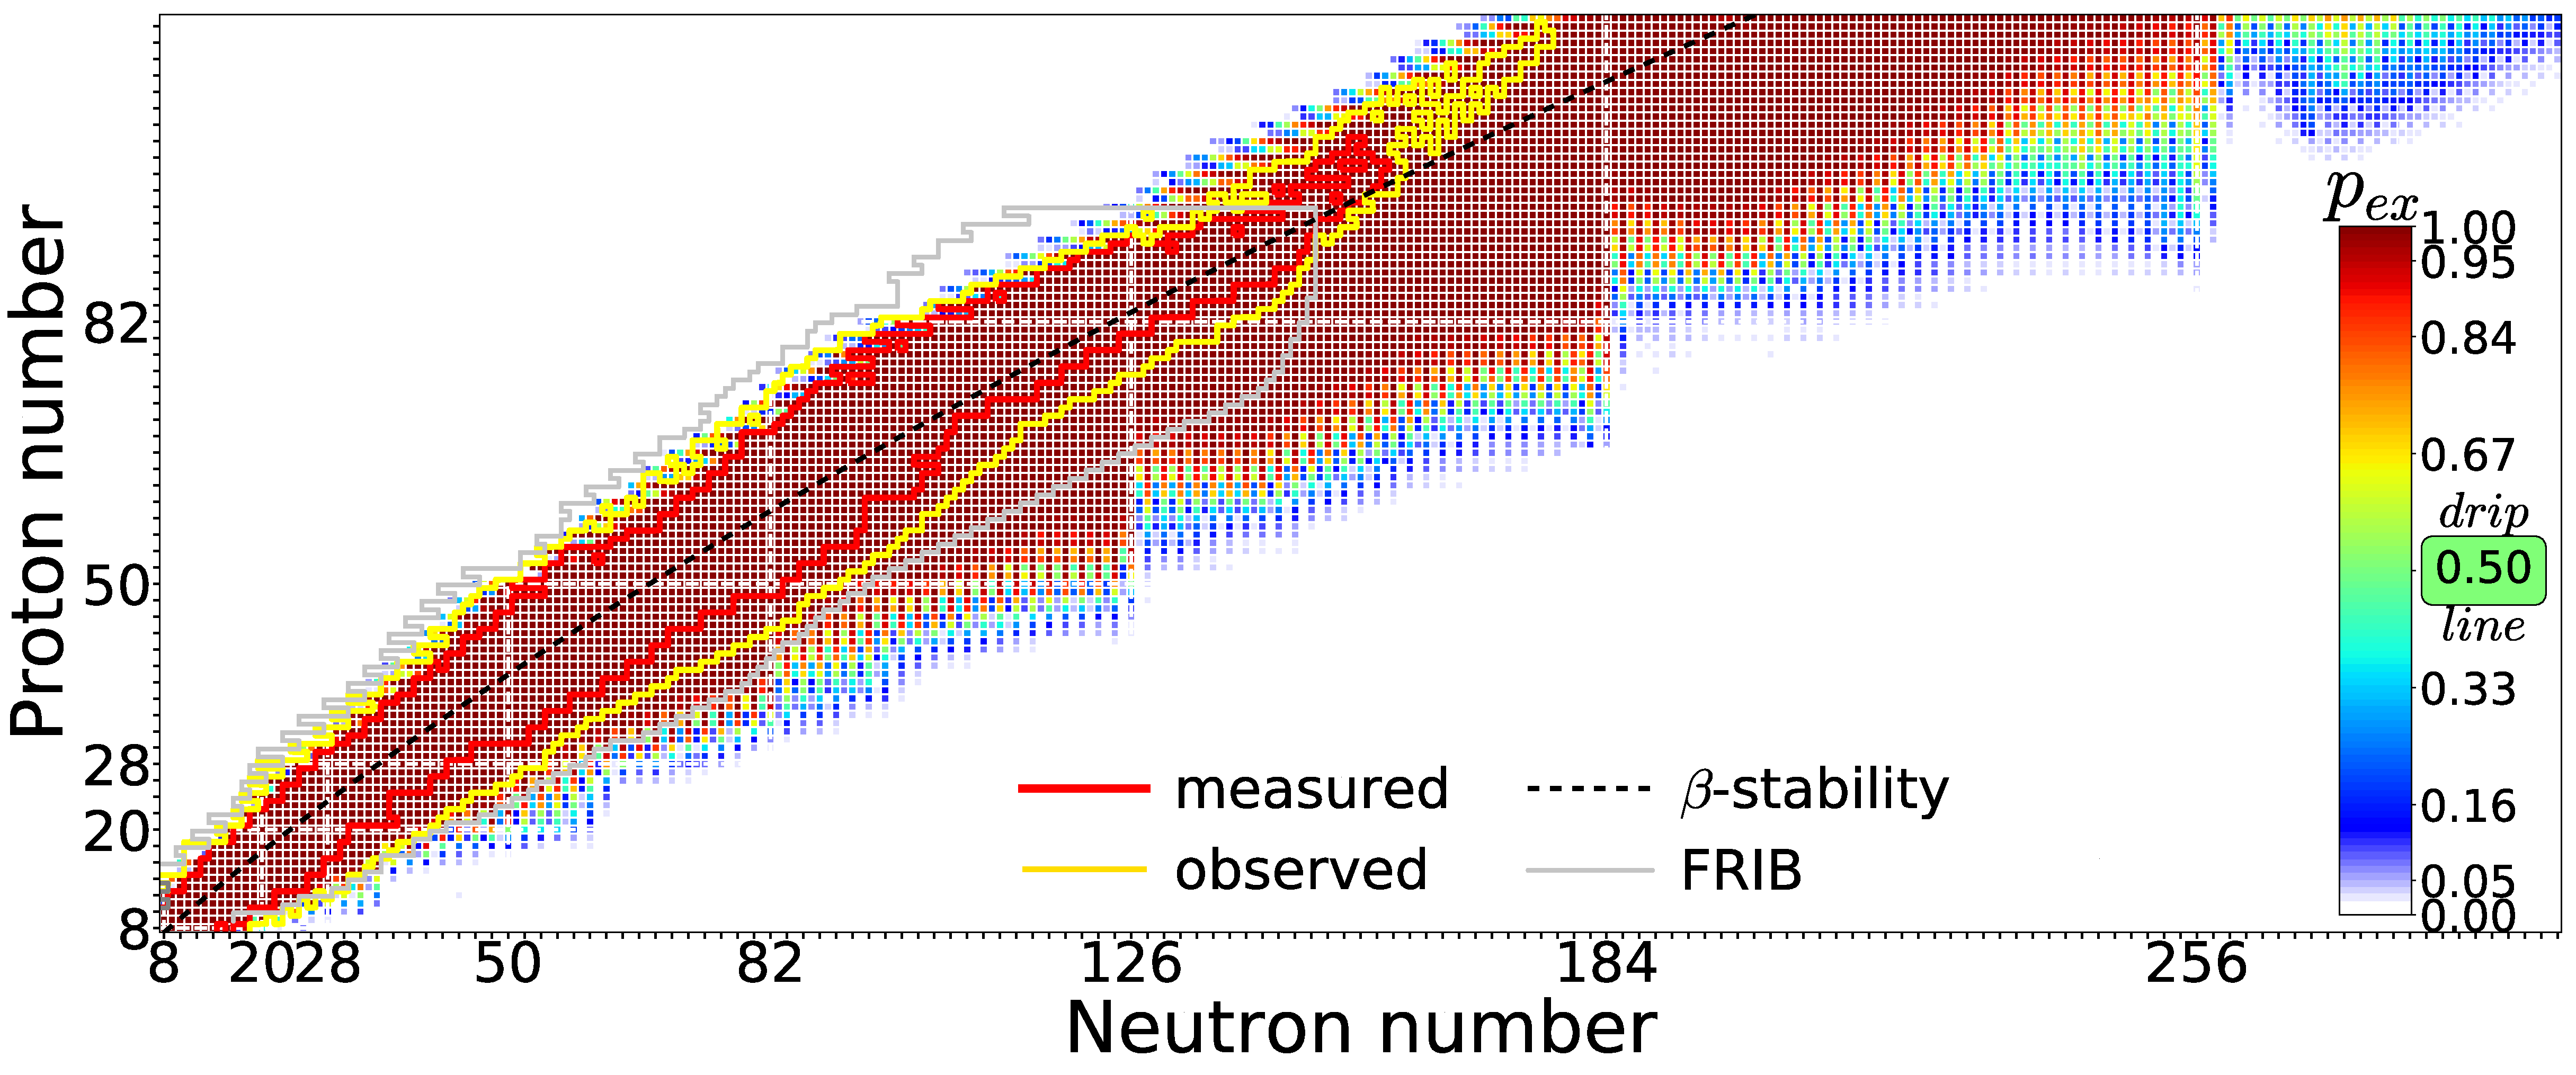
\includegraphics[width=\linewidth]{figures/Landscape.pdf}
\caption{
The quantified  landscape of nuclear existence obtained in our BMA calculations. For every nucleus with $Z,N \ge 8$ and $Z\le 119$
the probability that  the nucleus is bound with respect to proton and neutron decay, is marked.
The domains of nuclei which have been experimentally observed and whose separation energies have been  measured (and  used for training) are indicated together with 
the experimental reach of  FRIB.
}
\end{figure}

\clearpage
\newpage

\subsubsection{Statistical Aspects of Nuclear Mass Models}
\vspace{5mm}
\noindent
\fbox{\begin{minipage}{\linewidth}
\begin{description}
%%%
\item[Participants:] V. Kejzlar (g), L. Neufcourt (p),  W. Nazarewicz,  and P.-G.~Reinhard (Erlangen)
%%%
\item[Description:]  We study the information content of nuclear masses from the perspective of global models of nuclear binding energies. To this end, we employ a number of statistical methods and diagnostic tools, including BC, BMA, REG, PCA, and ECP  by considering discrepant mass domains for calibration. We show that  a quite dramatic parameter reduction can be achieved.
%%%
\item[FRIB relevance:] The use of statistical methodologies and diagnostic tools advocated in this work will be useful in further studies of nuclear models, both for the sake of understanding their structure and for practical applications pertaining to FRIB science.
%%%
\item[References:] {\it Statistical aspects of nuclear mass models}, V. Kejzlar L. Neufcourt, W. Nazarewicz,  and P.-G.~Reinhard, \href{https://arxiv.org/abs/2002.04151}{Submitted to the J. Phys. G Focus ISNET 2 Issue}.
\end{description}
%%%
\end{minipage}
}
\begin{SCfigure}[10][b]
\centering
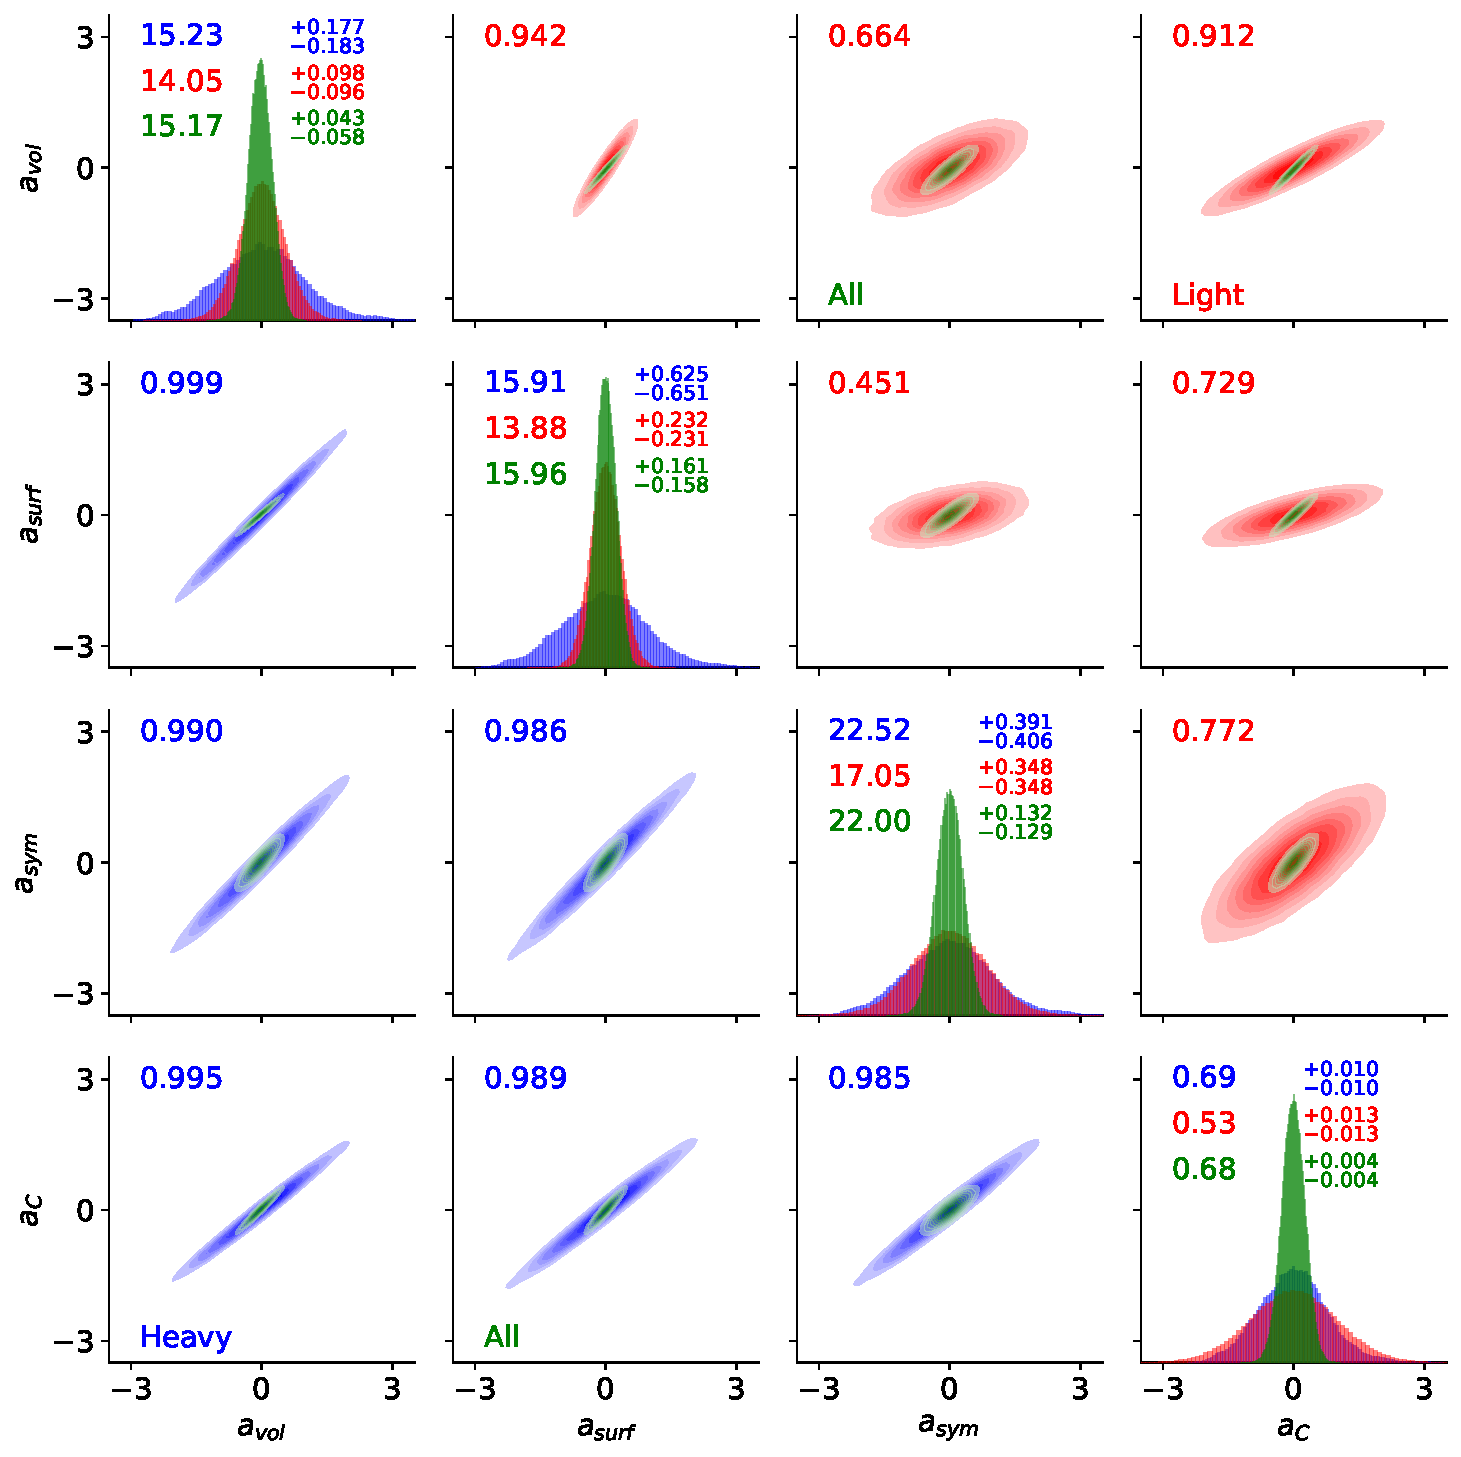
\includegraphics[width=0.7\linewidth]{figures/A_L_H_trace.pdf}
\caption{
Posterior distribution of the  parameters for three  liquid drop model
variants fitted on specific regions of the nuclear landscape.
The conditioning data were the binding energies of even-even nuclei divided into light ($Z<40$, $N<50$), heavy ($Z>50$, $N>80$), and intermediate nuclei (remaining 155 nuclei). Posterior mean and standard
deviation are indicated by numbers as well as correlation coefficients for all parameters.
}
\end{SCfigure}

\clearpage
\newpage



\subsubsection{Deep Learning and the Nuclear Many-Body Problem}
\vspace{5mm}
\noindent
\fbox{\begin{minipage}{0.96\linewidth}
\begin{description}
%%%
\item[Participants:] J. Hartley (g), J. Kim (g), O. Udiani (g), S. Bogner, H. Hergert, and M Hjorth-Jensen
%%%
\item[Description:] ML methods make it possible to tackle the curse of dimensionality and allow us to model quantum mechanical systems with less a priori knowledge. For complex many-body systems like nuclei (especially those at the limits of stability) or nuclear matter, this is a very interesting avenue to explore.  We have recently applied DL methods --- particular RNNs, LSTM and KRR --- to Similarity
Renormalization Group flows and the solution of Coupled Cluster theory, with a great deal of success. Our preliminary studies hold great promise for handling systems with large numbers of particles (including nuclear matter) or basis states (e.g. due to deformation or continuum coupling).
%%%
\item[FRIB relevance:]  Theoretical studies of nuclei at the limits of stability are a great challenge due to the large number of degrees of freedom. These systems are highly relevant for the scientific program of FRIB. Our early results also suggest connections between RG methods and Deep Learning that will contribute to a better understanding of Machine Learning methods.
%%%
\item[References:] {\it Recurrent Neural Networks and the Nuclear Many-body Problem}, in preparation
\end{description}
%%%
\end{minipage}
}
\begin{figure}[htb!]
\centering
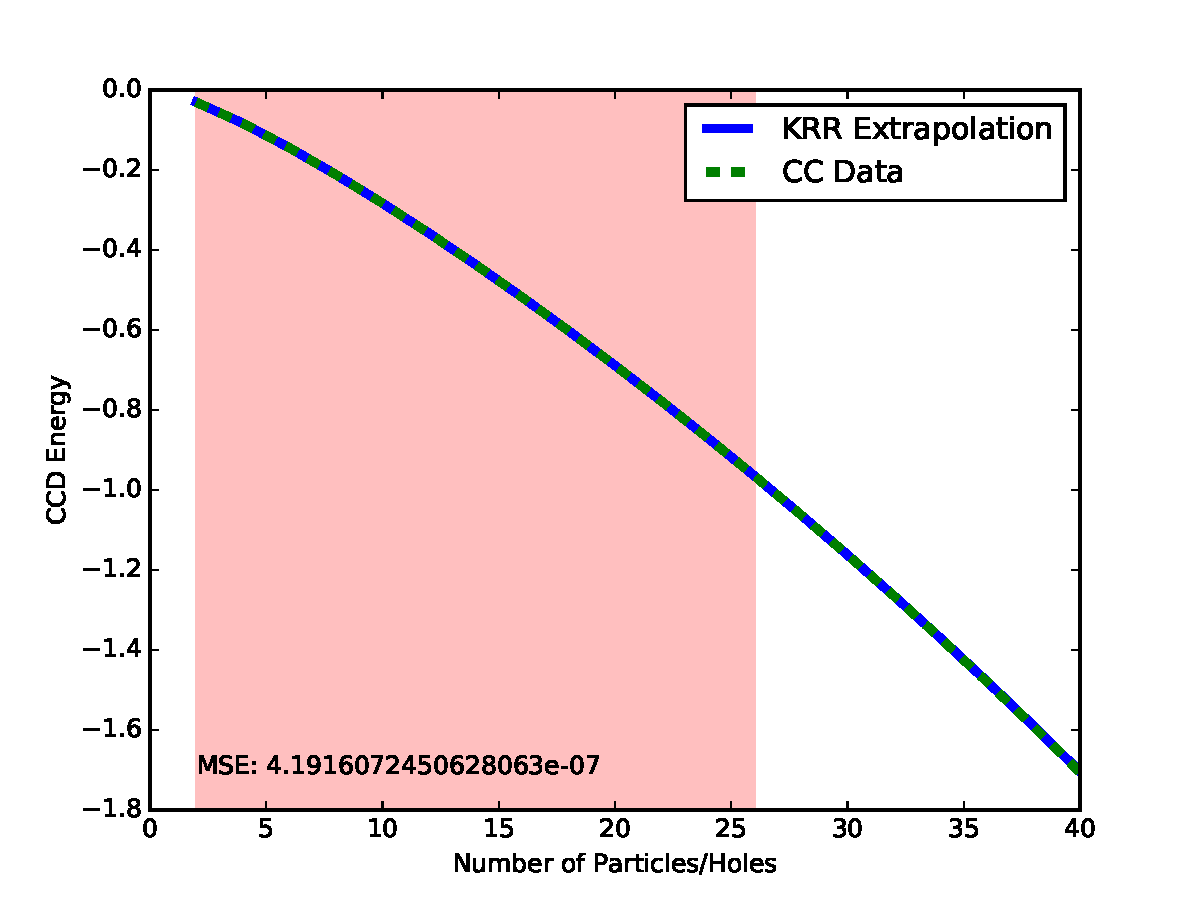
\includegraphics[width=0.75\linewidth]{figures/KRR_CC.pdf}
\vspace{-8pt}
\caption{Extrapolations to large numbers of interacting fermions for a pairing model using KRR methods on Coupled Cluster data.}
\end{figure}
\clearpage
\newpage

\subsubsection{Boltzmann Machines and the Nuclear Many-Body Problem}
\vspace{5mm}
\noindent
\fbox{\begin{minipage}{0.98\linewidth}
\begin{description}
%%%
\item[Participants:] J. Hartley (g), J. Kim (g), S. Bogner, and M Hjorth-Jensen
%%%
\item[Description:] We have recently started to explore several approaches based on DL algorithms, with an emphasis on NN and BM, with several promising results for interacting
many-fermion systems. Our applications
so far have been to systems of electrons confined to move in two or
three-dimensional regions (so-called quantum dots) and systems of
bosons (weakly and strongly interacting) using a mix of NN
based algorithms and variational quantum Monte Carlo approaches. We are in the process of extending these calculations
to nuclear physics problems.
%%%
\item[FRIB relevance:] The ability to study theoretically nuclei at the limits of stability is a great challenge due to the huge number of degrees of freedom. These systems are highly relevant for the scientific program of FRIB. 
%%%
\item[References:] {\it Solving Many-Body Problems with Boltzmann Machines}, in preparation
\end{description}
%%%
\end{minipage}
}
\begin{figure}[htb!]
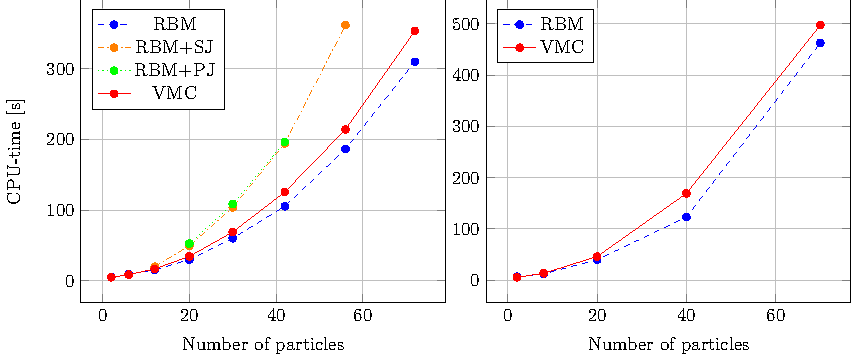
\includegraphics[width=\linewidth]{figures/quantumdots.pdf}
\caption{Ground state energies for systems of quantum dots.}
\end{figure}

\clearpage\newpage

\subsubsection{Emulators for the Nuclear Many-Body Problem}
\vspace{5mm}
\noindent
\fbox{\begin{minipage}{0.98\linewidth}
\begin{description}
%%%
\item[Participants:] D. Lee
%%%
\item[Description:] In applications of machine learning and uncertainty quantification to first principles nuclear many-body theory, one important tool is a fast and accurate emulator that removes the need for repeatedly performing computationally-expensive calculations.  We show that eigenvector continuation can fill this role quite nicely.  In addition to its applications as an emulator, eigenvector continuation can also be trained as a machine learning method for the quantum many-body problem using optimized variational subspaces. 
%%%
\item[FRIB relevance:] One of the fundamental challenges in FRIB science is understanding the connection between microscopic nuclear forces and nuclear structure.  Having a fast and accurate emulator makes it possible to apply machine learning and uncertainty quantification to uncover the correlations between nuclear forces and structure.
%%%
\item[References:] {\it Eigenvector Continuation as an Efficient and Accurate Emulator for Uncertainty Quantication in Nuclear Systems}, S. König, A. Ekström, K. Hebeler, D. Lee, and A. Schwenk, \href{https://arxiv.org/abs/1909.08446}{arXiv:1909.08446, submitted}.
\end{description}
%%%
\end{minipage}
}
\begin{figure}[htb!]
\centering
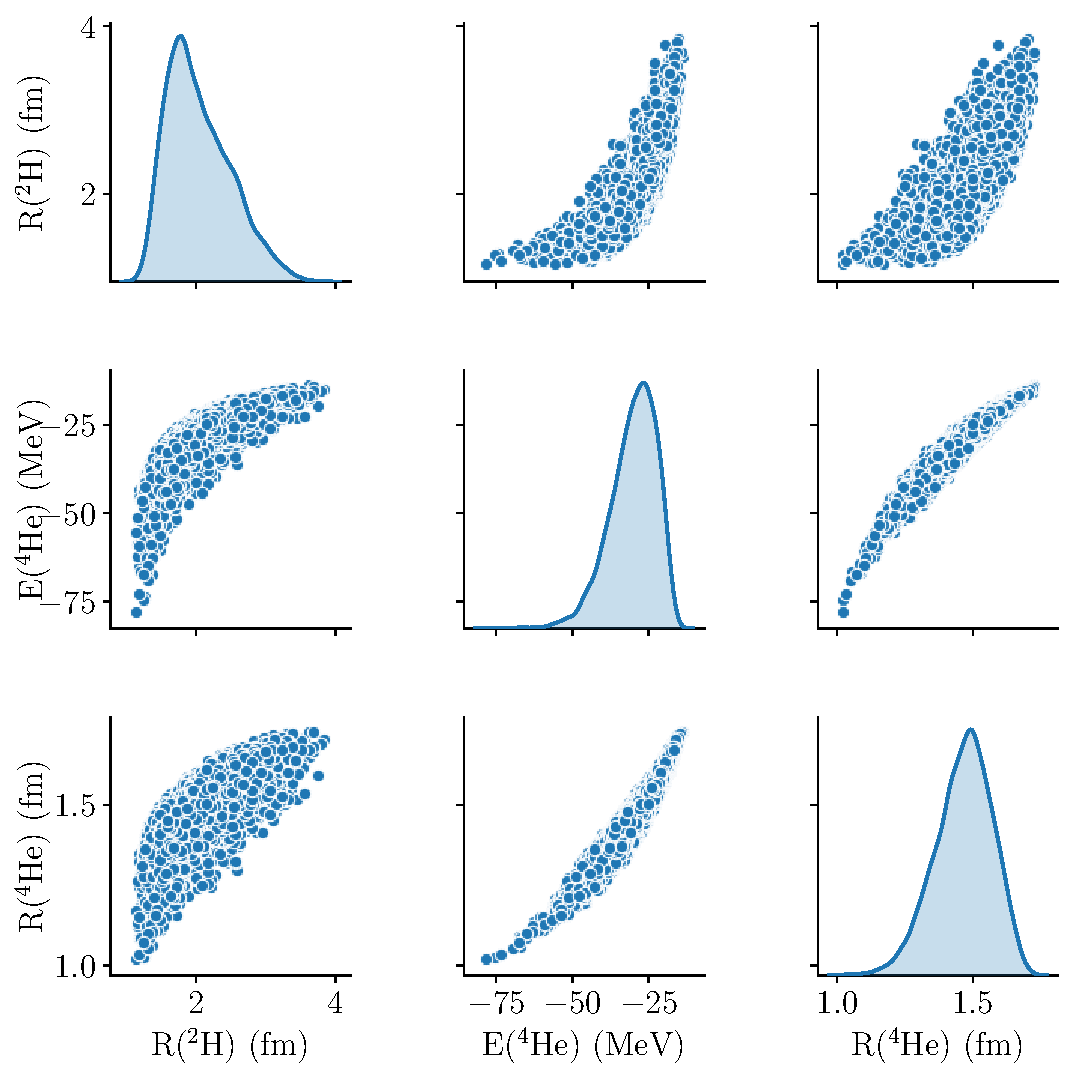
\includegraphics[width=8cm]{figures/few_body_grid_subset.pdf}
\caption{Correlations among several observables for $^2$H and $^4$He computed using eigenvector continuation.}
\end{figure}

\clearpage\newpage

\subsubsection{Machine Learning Multi-Nucleon Correlations}
\vspace{5mm}
\noindent
\fbox{\begin{minipage}{0.98\linewidth}
\begin{description}
%%%
\item[Participants:] J. Bonitati (g), G. Given (g), and D. Lee
%%%
\item[Description:] We are using BM to uncover and quantify multi-nucleon correlations in supercomputer lattice data obtained from lattice simulations of atomic nuclei.  The work involves the development of new algorithms to bypass the computational bottleneck of computing the overall normalization of the partition function and dealing with negative weight configuration produced in the quantum simulations.
%%%
\item[FRIB relevance:] We would like to understand the microscopic origins of nuclear clustering across the nuclear chart.  As the phenomenon of clustering is accentuated near open thresholds, these studies are of direct relevance to FRIB science.
%%%
\item[References:] {\it Machine Learning Multi-Nucleon Correlations from First Principles}, J. Bonitati, G. Given, Da. Lee, and D. Lee, in preparation.
\end{description}
%%%
\end{minipage}
}
\begin{figure}[htb!]
\centering
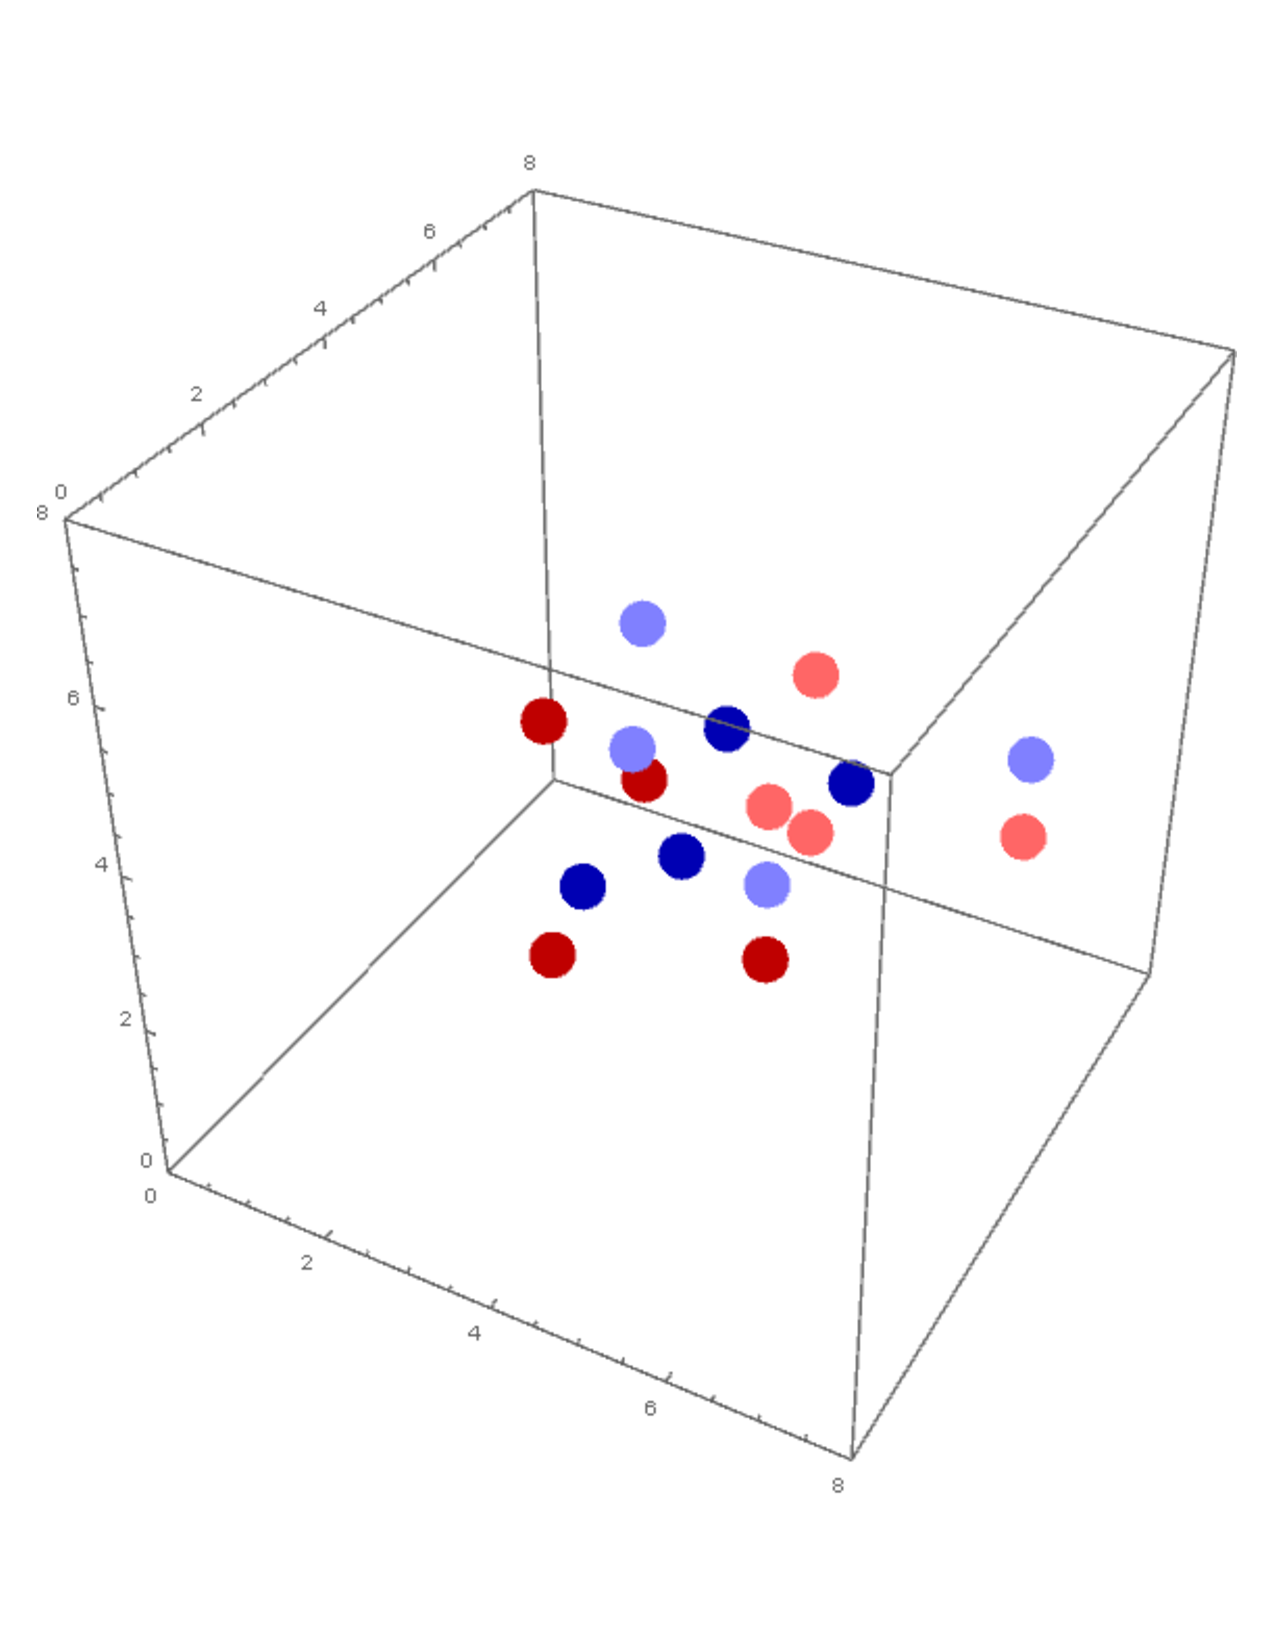
\includegraphics[width=7cm]{figures/training_data.pdf}
\caption{Sample training data used for machine learning multi-nucleon correlations in $^{16}$O.}
\end{figure}




\subsubsection{Machine Learning Algorithms for Hadron Correlators from Lattice QCD}
\vspace{5mm}
\noindent
\fbox{\begin{minipage}{0.98\linewidth}
\begin{description}
%%%
\item[Participants:] G. Pederiva (g), A. Shindler
%%%
\item[Description:] Lattice QCD calculations
  are an effective tool to probe the dynamics of quarks and gluons at low energies.
  However, these calculations require large computational capabilities,
  for example when computing the building block of any hadron correlation function:
  the quark propagator.
  We are studying the feasibility of using ML,
  in particular algorithms based on Boosted Decision
  Trees and  ANN,
  to reduce the cost of the iterative solvers for quark propagator
  by relating solutions to the system computed at different precision.
%%%
\item[FRIB relevance:] Understanding the nuclear structure starting
  from the strong interactions between quarks and gluons and between nucleons,
  is one of the main research thrusts of FRIB.
  Reducing the computational cost of quark propagator
  calculations could effectively lead to a precise determination of 
  multi-nucleon correlators and nucleon scattering phase shifts with current
  state-of-the-art hardware and software.
%%%
\item[References:] {\it Machine Learning Algorithms for Hadron Correlators from Lattice QCD},
  G. Pederiva, A. Shindler, in preparation  
\end{description}
%%%
\end{minipage}
}

\begin{figure}[htb!]
\centering
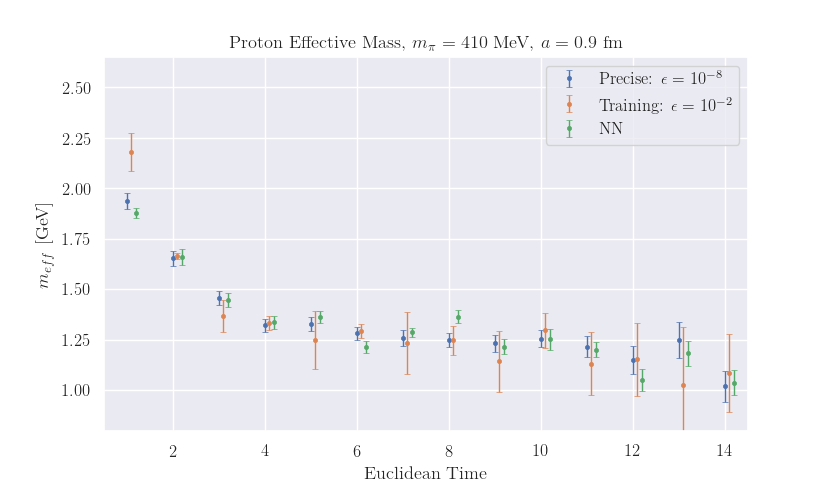
\includegraphics[width=\textwidth]{figures/eff_mass.png}
\caption{Example of proton effective mass plot with data from a precise calculation using a small stopping criterion $\epsilon=10^{-8}$ in the BiCGStab solver, a training set using a much larger $\epsilon = 10^{-2}$, and the NN results for the same data.}
\end{figure}




\subsubsection{Establishing a statistical approach to nuclear reactions}
\vspace{5mm}
\noindent
\fbox{\begin{minipage}{0.98\linewidth}
\begin{description}
%%%
\item[Participants:] F.M. Nunes, A. Lovel (g), G. King (u), L. Neufcourt (p)
%%%
\item[Description:] The few-body group has been exploring statistical methods in nuclear reactions. 
In 2018 we compared, directly and systematically, the frequentist and Bayesian approaches to quantifying uncertainties in direct nuclear reactions. Our study demonstrated that the uncertainties on the reaction observables considered  within the Bayesian approach  represent reality more accurately than the much narrower uncertainties obtained using the standard frequentist approach.
%%%
\item[FRIB relevance:] To interpret reaction data from FRIB, we need to reliably quantify the uncertainties in the nuclear theories used. 
%%%
\item[References:] G. B. King, A. E. Lovell, L. Neufcourt, and F. M. Nunes,
\href{https://journals.aps.org/prl/abstract/10.1103/PhysRevLett.122.232502}{Phys. Rev. Lett. 122, 232502 (2019)}.
\end{description}
%%%
\end{minipage}
}
\begin{figure}[htb!]
\centering
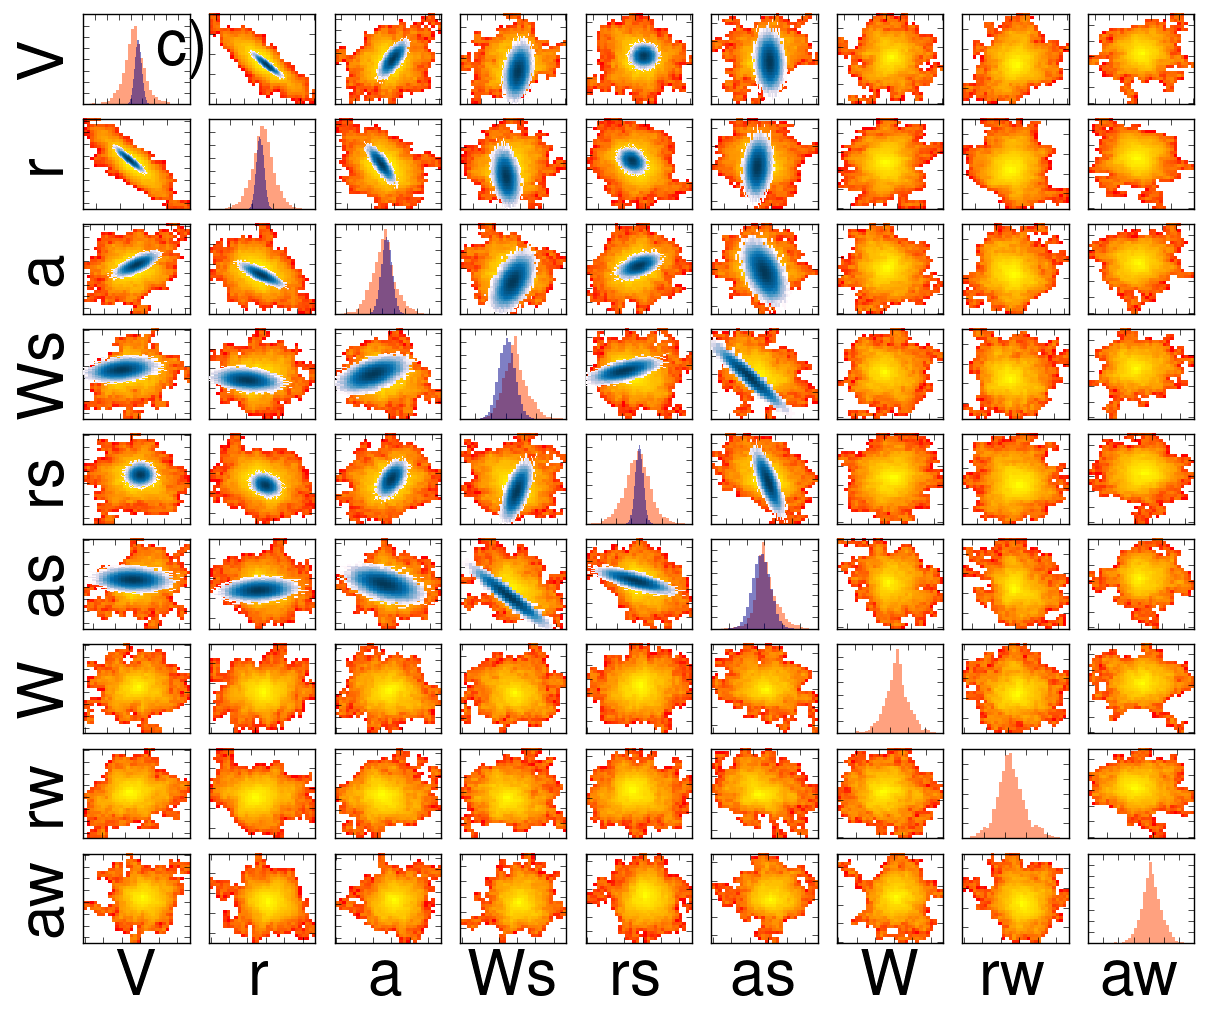
\includegraphics[width=0.63\linewidth]{figures/48cap25-100k-scatter.png}
\caption{Posterior distributions for the parameters (diagonal) and scatter plots for the correlations between parameters: Bayesian are shown in shades of orange and frequentist in shades of blue for $^{48}$Ca(p,p) at 25 MeV. Depths are in MeV and radii and difuseness are in fm.}
\end{figure}


\subsubsection{Bayesian approach to nuclear reactions and Experimental Design}
\vspace{5mm}
\noindent
\fbox{\begin{minipage}{0.98\linewidth}
\begin{description}
%%%
\item[Participants:] F.M. Nunes, A. Lovell (g), G. King (u) and M. Catacora-Rios (g)
%%%
\item[Description:]  

In recent work we study the uncertainties of optical model parameters and its dependence on the angular grid of the differential cross section, the inclusion of cross section data at nearby energies, and changes in the experimental error bars.  We also study the effect on the resulting uncertainty when total reaction cross sections are included in the fitting procedure. 

In the last years, we have been expanding our methods to include the PCA and BML to identify the optimum experimental conditions and the best combination of observables to reduce the uncertainty on the resulting cross sections. Once this is completed, we plan to use these statistical tools to make model comparisons and eventually, if it makes sense, to perform BMA
\item[FRIB relevance:] To plan reactions measurements at FRIB it is important to know what are the optimum conditions and the optimum observables (or combination of observables) that provide maximum information content. 
%%%
\item[References:]  M. Catacora-Rios, G. B. King, A. E. Lovell, and F. M. Nunes
\href{https://journals.aps.org/prc/abstract/10.1103/PhysRevC.100.064615}{Phys. Rev. C 100, 064615 (2019)}.
\end{description}
%%%
\end{minipage}
}
\begin{SCfigure}[10][b]
\centering
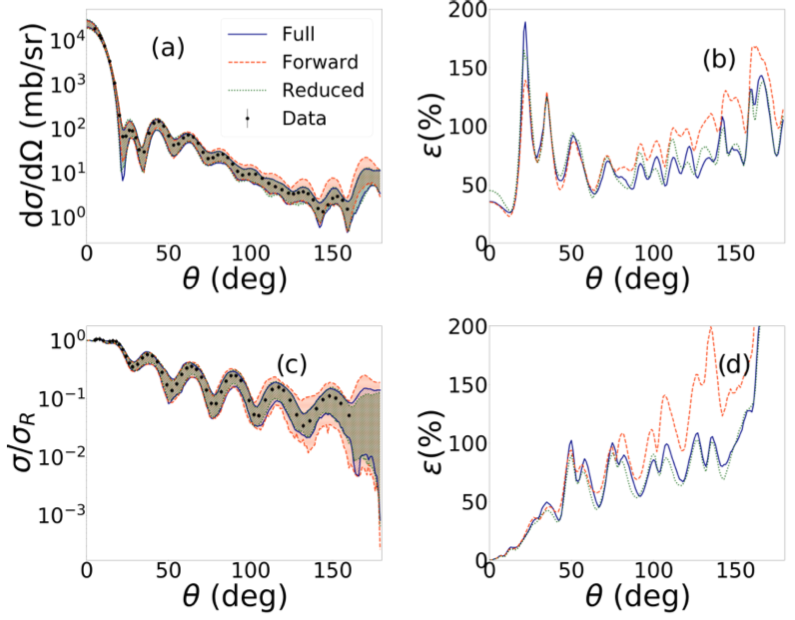
\includegraphics[width=0.7\linewidth]{figures/208Pbdpdata.png}
\caption{A comparison of results using the full angular range (blue solid line)  with those where only forward angles are used (orange dashed) or half of the data points are considered (green dotted) for $^{208}$Pb(n,n) at 30 MeV 95$\%$ confidence intervals and percentage uncertainty plot.}
\end{SCfigure}

\clearpage\newpage

\clearpage
\newpage
\subsubsection{Bayesian approach to constrain parameters of the Equation of State}
\vspace{5mm}
\noindent
\fbox{\begin{minipage}{0.98\linewidth}
\begin{description}
\item[Participants:] C.Y. Tsang (g), W.G. Lynch, M.B. Tsang
%%%
\item[Description:] 
Transport model theory predicts that ratios of neutron and proton energy spectra provide constraints on the density and momentum dependencies of the isovector mean-field potential. To extract the parameters of the equation of state, ($\rho$, S($\rho$), $m_n^*$, $m_p^*$ corresponding to density,  symmetry energy,  neutron and proton effective masses, respectively), we compare single and double n/p ratios obtained from central collisions of $^{112}$Sn+$^{112}$Sn and $^{124}$Sn+$^{124}$Sn at 120 MeV/u to a transport model calculations. Using Bayesian analysis which samples millions of parameter sets, we obtain the 1 and 2 sigma contours of the density dependence of the symmetry energy (see figure). For the effective mass, the results are more ambiguous. We need better data especially at higher kinetic energy where sensitivity to the effective mass splitting is larger.
%%%
\item[FRIB relevance:] Determining the nuclear equation of state is an important component of the FRIB science.
%%%
\item[References:] { {\it Constraining the symmetry energy with heavy-ion collisions and Bayesian analyses}, P. Morfouace, C.Y. Tsang, Y.Zhang, W.G. Lynch, M.B.Tsang, et al., \href{https://doi.org/10.1016/j.physletb.2019.135045}{Phys. Lett. B 799 135045 (2019)} }.
\end{description}
%%%
\end{minipage}
}

\begin{figure}[htb!]
\centering
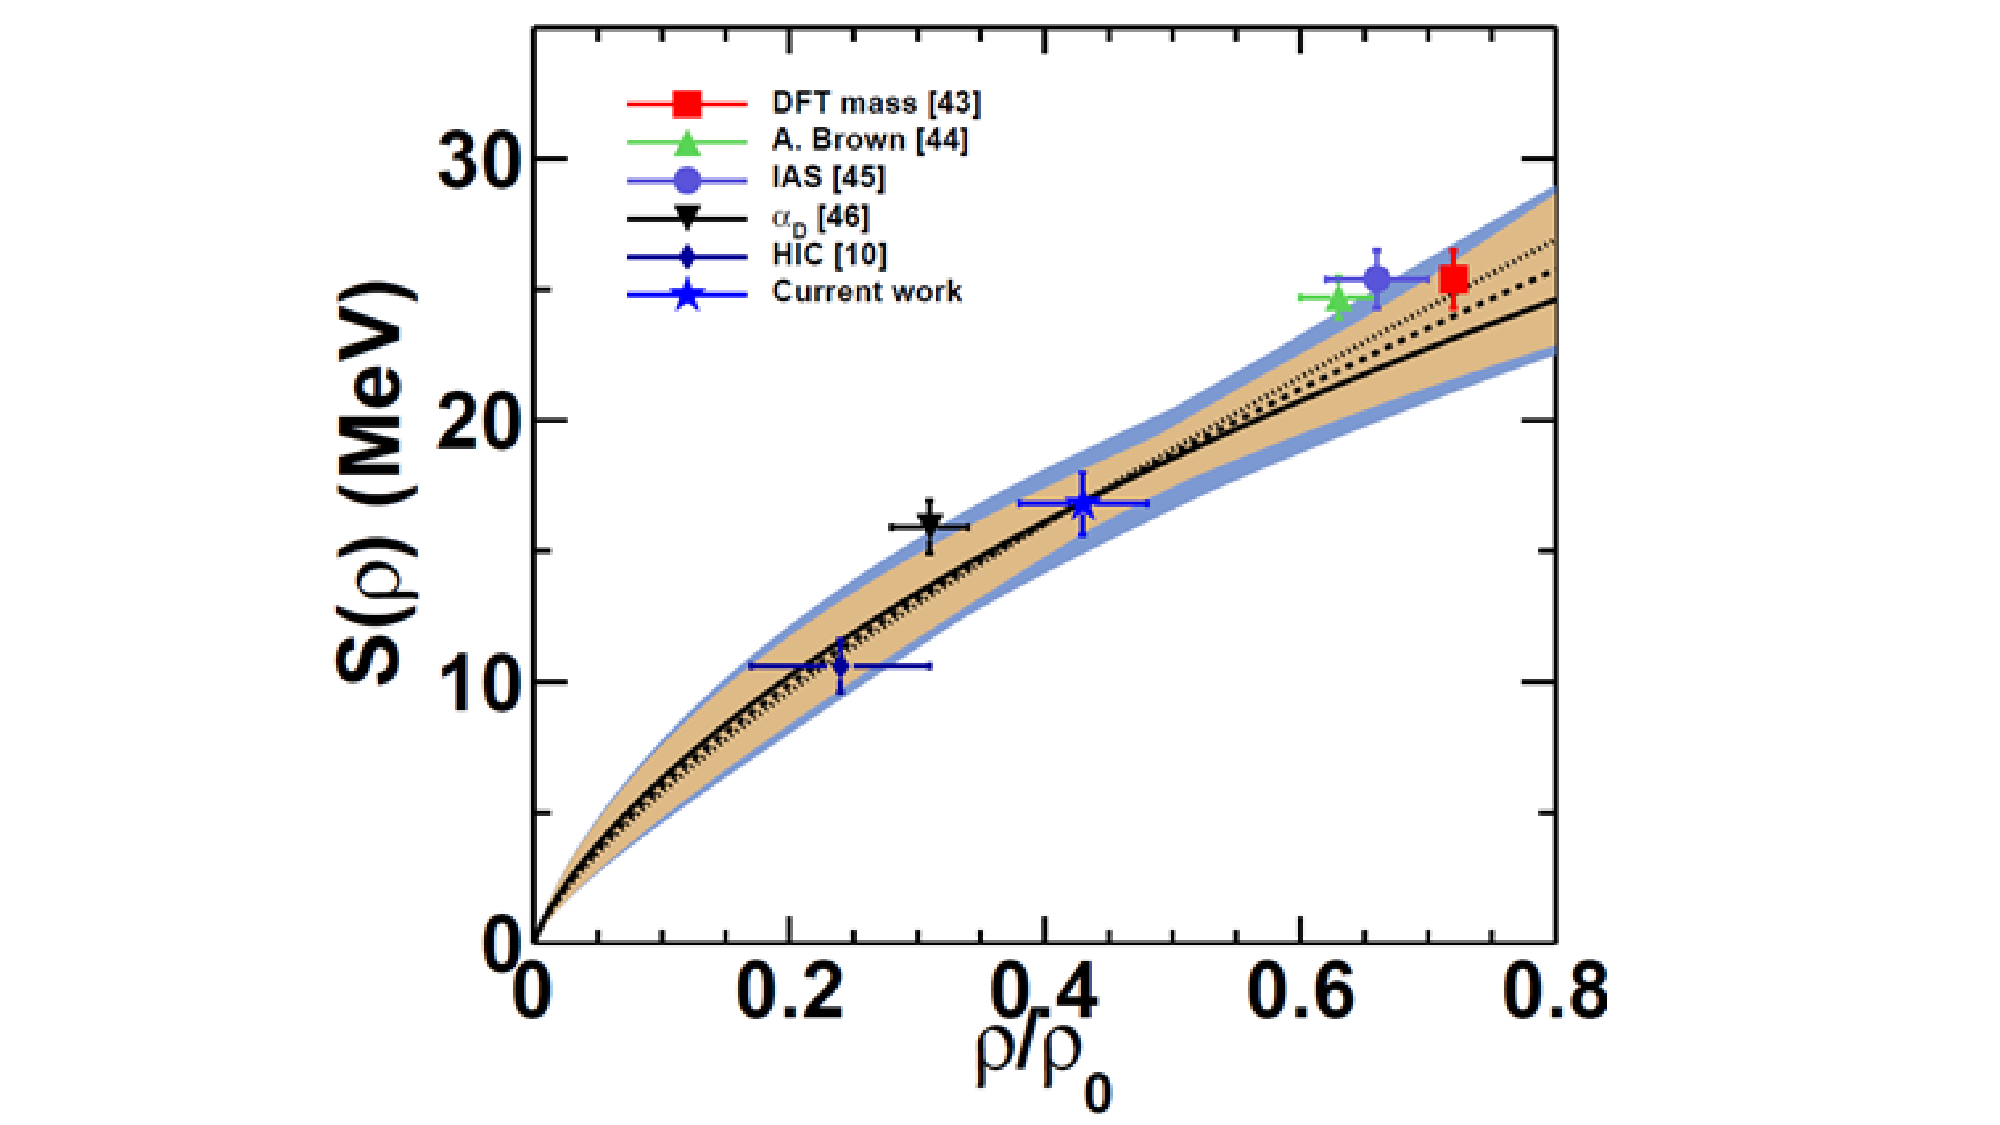
\includegraphics[width=0.87\linewidth]{figures/Pierre_contour.pdf}
\caption{
Density dependence of the symmetry energy S($\rho$).  The color areas correspond to the symmetry energy
versus density of the $1\sigma$ (brown) and $2\sigma$ (blue) contours from Bayesian analysis of single and double ratios of central collisions of $^{112}$Sn+$^{112}$Sn and $^{124}$Sn+$^{124}$Sn at 120 MeV/u. Symbols are data from different experiments.
}
\end{figure}
\clearpage
\newpage

\subsubsection{Bayesian approach to study the correlations of neutron star deformability and Equation of State parameters}
\vspace{5mm}
\noindent
\fbox{\begin{minipage}{0.98\linewidth}
\begin{description}
\item[Participants:] C.Y. Tsang (g) and M.B. Tsang
%%%
\item[Description:] 
We use a Bayesian inference analysis to explore the sensitivity of Taylor expansion parameters of
the nuclear equation of state (EOS) to the neutron star dimensionless tidal deformability ($\Lambda$) obtained
from the neutron star merger event GW170817. To avoid correlations between the expansion
parameters, we use a prior distributions based on a recently published meta-modeling approach.
However, we find that assumptions in the prior distribution strongly
influence the constraints on $\Lambda$.
The sensitivity study is extended beyond the canonical neutron star with 1.4 solar mass. For neutron
star with mass < 1.6 solar mass, $L_{sym}$ and $K_{sym}$ are highly correlated with the tidal deformability.
For more massive neutron stars, the tidal deformability is more strongly correlated with higher order
Taylor expansion parameters. 
%%%
\item[FRIB relevance:] Investigating dense nuclear matter on earth and in heavens is one of the major objectives in  FRIB science.
%%%
\item[References:] { {\it Insights on Skyrme parameters from GW170817}, C. Y. Tsang, M. B. Tsang, P. Danielewicz, F. J. Fattoyev,and W. G. Lynch, \href{https://doi.org/10.1016/j.physletb.2019.05.055}{Phys. Lett. B 796 1 (2019)} }.
\end{description}
%%%
\end{minipage}
}

\begin{figure}[htb!]
\centering
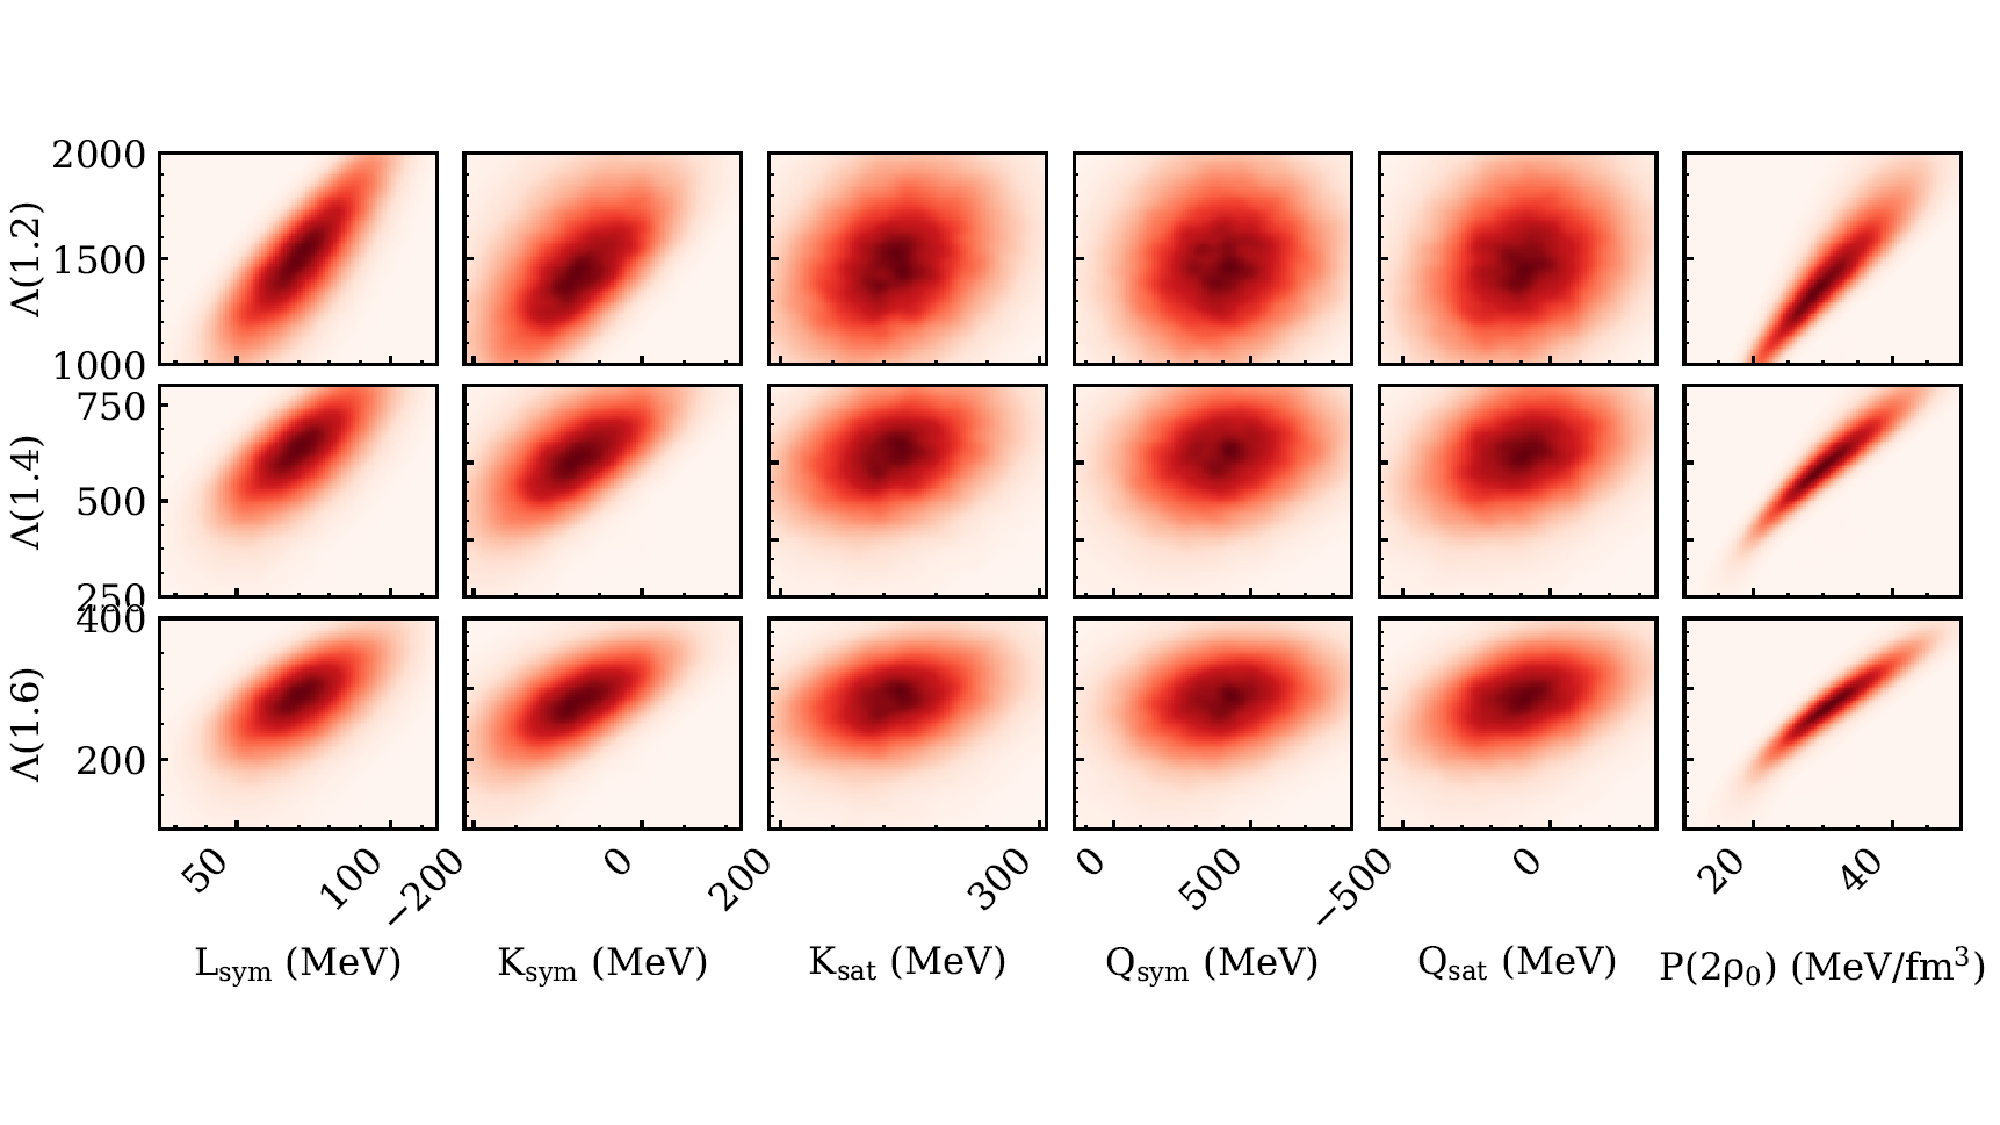
\includegraphics[width=1.0\linewidth]{figures/lamda_LKQ.pdf}
\caption{
Bivariate distributions between neutron star deformabilities ($\Lambda$) and Taylor expansion parameters, $L$, $K$, $Q$ and pressure at twice normal nuclear matter density, $P(2\rho_0)$ for neutron stars with different masses.
}
\end{figure}

\subsubsection{Applying Machine Learning to Bayesian Emulators}
\vspace{5mm}
\noindent
\fbox{\begin{minipage}{0.98\linewidth}
\begin{description}
\item[Participants:] S. Pratt
%%%
\item[Description:]
Equation-of-state analyses require rigorous comparison of large heterogeneous data sets to sophisticated models, using input from nuclear structure, heavy-ion collisions and astrophysical observations. Due to the numerical expense of theoretical models model emulators have been employed to explore the highly multi-dimensional model space. Emulators approximate the full model by interpolating from a modest number of full-model runs, but even with an emulator these studies push the limits of large computing facilities. For example, the Bayesian exploration summarized in the figure below involved 1200 full model runs over a 14-dimensional parameter space. One must choose how many full model runs to perform, and at which points, and with what accuracy. If the runs require a sampling of events, should one sample fewer events or use the computational budget to explore more points in parameter space.  Machine learning provides a natural strategy for guiding and optimizing these studies. Such optimizations might save large amounts of computational expense, and make certain studies tenable that might otherwise be inconceivable.

%%%
\item[FRIB relevance:] Data from heavy-ion collisions and structure experiments from FRIB will both play a critical role in equation of state analyses.
%%%
\item[References:] { S.~Pratt, E.~Sangaline, P.~Sorensen and H.~Wang,
  {\it Constraining the Eq. of State of Super-Hadronic Matter from Heavy-Ion Collisions},
  \href{https://journals.aps.org/prl/abstract/10.1103/PhysRevLett.114.202301}{Phys.\ Rev.\ Lett.\  {\bf 114}, 202301 (2015) }}.
\end{description}
%%%
\end{minipage}
}
\begin{figure}[htb!]
\centering
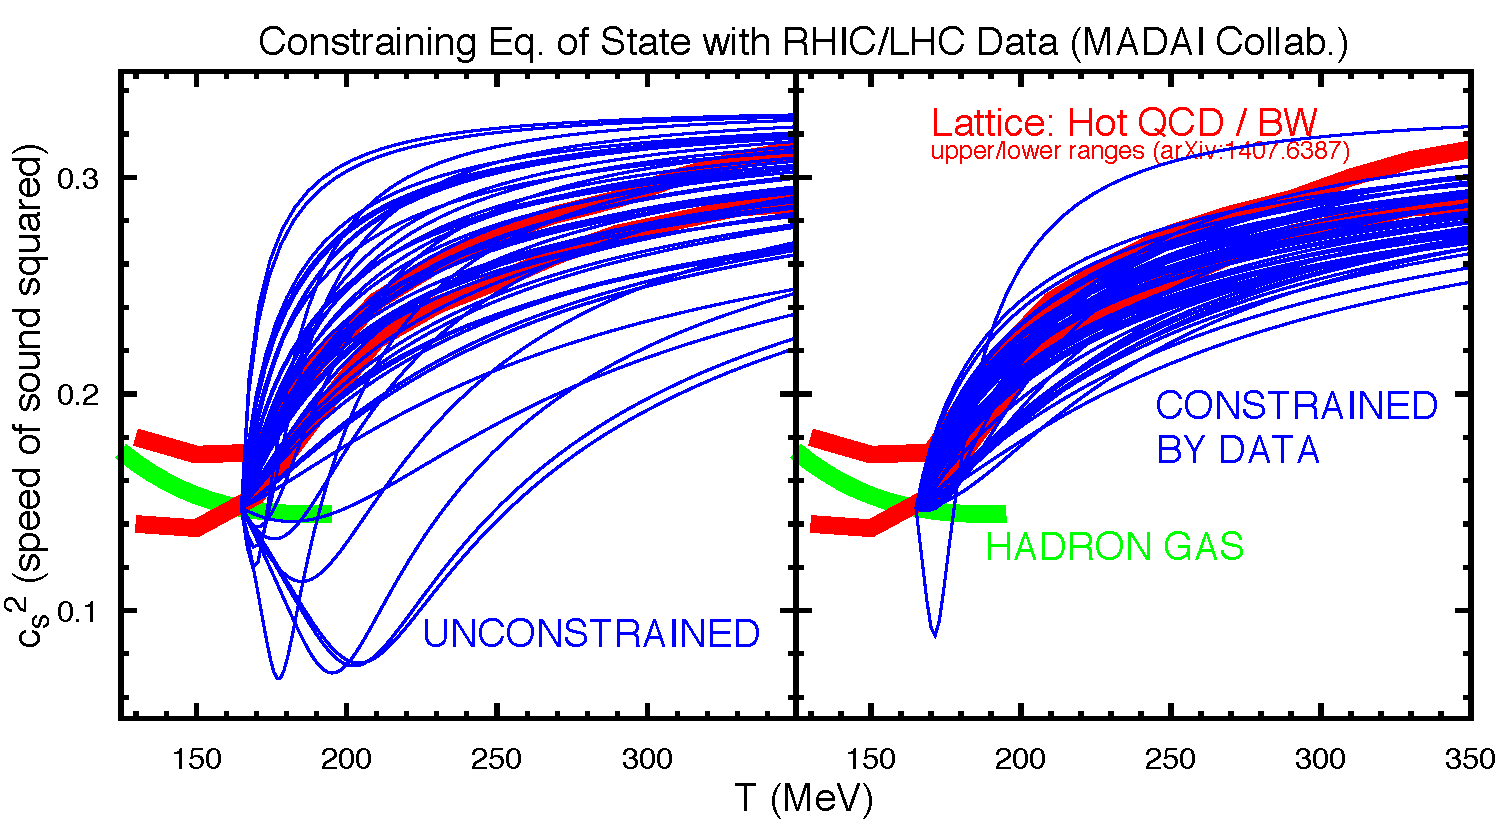
\includegraphics[width=0.75\linewidth]{figures/madai_rhiclhc.pdf}
\caption{
The equation of state derived from a 14-parameter Bayesian analysis. Eq.s of state from a random assortment of parameters (left panel, Bayesian prior) are compared to those weighted by the Bayesian likelihood(right panel).
}
\end{figure}

\subsubsection{Bayesian Inference of Symmetry Energy Characteristics from Nucleon Induced Reactions}
\vspace{5mm}
\noindent
\fbox{\begin{minipage}{0.98\linewidth}
\begin{description}
\item[Participants:] Pawel Danielewicz
%%%
\item[Description:]
Symmetry energy quantifies changes in the nuclear equation of state with changes in the neutron-proton imbalance.  Knowledge of the symmetry energy as a function of density is essential for extrapolating from nuclear laboratory measurements to properties of neutron stars.  The symmetry energy at saturation and subsaturation densities affects relative distribution of neutrons and protons in nuclei and isospin structure of the Lane optical potential that governs nucleon elastic scattering and quasielastic charge exchange reactions.  By simultaneously analyzing data from nucleon elastic scattering and nucleon quasielastic charge exchange reactions for the same targets and combining these analyses with results of other data on isospin characteristics of nuclei, in layers of Bayesian inference, Danielewicz et al. placed constraints on stiffness of the symmetry energy.

%%%
\item[FRIB relevance:] Inferences from measurements at FRIB, pertaining to the nuclear equation of state, need to be combined in a rational manner with inferences from data collected elsewhere, often in completely different measurements, and from astronomical observations.
%%%
\item[References:] { Pawel Danielewicz, Pardeep Singh and Jenny Lee,
  {\it Symmetry Energy III: Isovector Skins},
  \href{https://www.sciencedirect.com/science/article/pii/S0375947416302895}{Nucl.\ Phys.\ A {\bf 958}, 147 (2017) }}.
\end{description}
%%%
\end{minipage}
}
\begin{figure}[htb!]
\centering
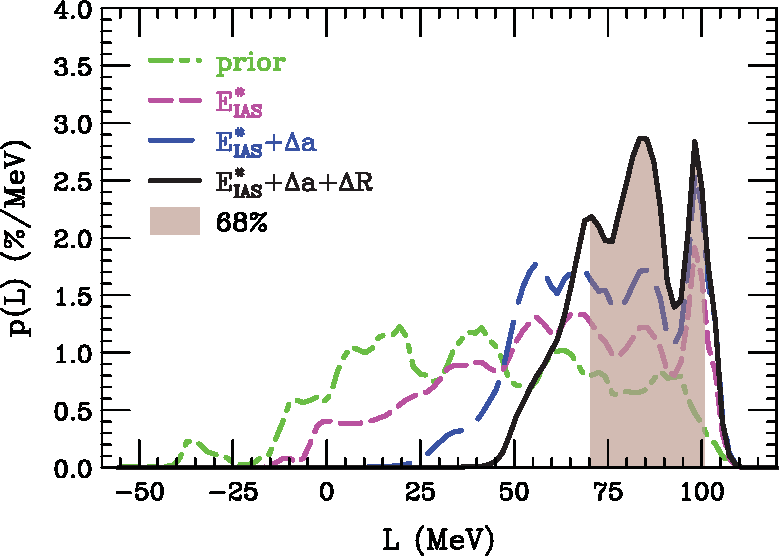
\includegraphics[width=0.75\linewidth]{figures/PL.pdf}
\caption{
Evolution of likelihood for the stiffness of symmetry energy $L$ as more data are taken into consideration.
}
\end{figure}


\clearpage
\newpage

\subsection{Applications}
\subsubsection{Add title}
\vspace{5mm}
\noindent
\fbox{\begin{minipage}{0.96\linewidth}
\begin{description}
%%%
\item[Participants:] Names%%%
\item[Description:]
%%%
\item[FRIB relevance:] 
%%%
\item[References:] {\it To be added}, in press/preparation/ or published 
\end{description}
%%%
\end{minipage}
}
\begin{figure}[htb!]
\centering
\caption{To be added}
\end{figure}
\clearpage
\newpage



\section{Education and Workforce}

There are only 26,000 AI researchers currently in the US. This is estimated to represent only a fifth of the current demand. There is an urgent need for training in AI, at a variety of educational levels and for diverse audiences. To this end, beyond our research efforts, we develop a range of outreach, recruitment, and educational activities. These activities will serve to raise interest in AI-related fields. We aim to retain talented students in AI-related fields and to help them to secure employment in a wide range of careers, thus ensuring that the new techniques and concepts developed at FRIB are widely disseminated.


\begin{itemize}

\item In order to develop education and training efforts that target AI and ML related methods applied to Nuclear Physics, in 2019 we  organized a four day long  \href{https://indico.frib.msu.edu/event/16/timetable/?view=standard}{FRIB-TA workshop} on {\it ML methods in Nuclear physics} at  NSCL/FRIB, with more than 100 participants.

\item In 2020 several of us (Bazin, Hjorth-Jensen and Liddick) will teach a three-week long Nuclear Talent course at ECT*  on \href{https://www.ectstar.eu/node/4472}{Machine Learning and Data Analysis applied to nuclear physics}. 


\item From spring 2020 (April and May, and planned to be repeated on an annual basis) we will host and run intensive courses on ML, Bayesian inference, and statistical data analysis for students and faculty in theoretical and experimental nuclear physics. The aim is to develop a large amount of material with lectures notes, videos, projects and hands-on material that can serve the whole nuclear Physics community. An example of possible material can found at \href{https://compphysics.github.io/MachineLearning/doc/web/course.html}.  The format of the course is similar to a Nuclear TALENT course.

\item
We initiated the series of meetings on {\it Enhancing the interaction between nuclear experiment and theory through information and statistics} \href{https://iopscience.iop.org/journal/0954-3899/page/ISNET}{(ISNET)}.  The next ISNET-8 will be held at FRIB during  Dec. 14-17th, 2020.

\end{itemize}

\clearpage
\newpage

%%%%%%%%%%%%%%%%%%%%%%%%%%%%%% future %%%%%%%%%%%%%%%%%%%%%%%%%%%%%%%%%%%%%%%%%%%%
\section{Appendix: Anticipated projects}

\subsection{Detectors}
\subsubsection{Particle reconstruction of Time Projection Chamber}

\vspace{5mm}
\noindent
\fbox{\begin{minipage}{0.98\linewidth}
\begin{description}
%%%
\item[Participants:] C.Y. Tsang (g),  W.G. Lynch, M.B. Tsang
%%%
\item[Description:] To investigate the ``nature of neutron-rich matter in the cosmos and on earth'' is one of the scientific objectives laid out in the 2015 NSAC Long Range Plan. With the energy and the availability of rare isotope beams, FRIB and FRIB400 are poised to study the Equation of State of asymmetric matter. One observable to study the EoS is to compare the relative emission of members of isospin multiplets, e.g. $\pi^-$ vs. $\pi^+$, $n$ vs. $p$, $t$ vs. $^3\mathrm{He}$, etc., which experience symmetry potentials and symmetry forces of opposite sign. Time projection chamber (TPC) provides large coverage to detect charged particles including pions emitted in heavy ion collisions (See figures). However, with mean multiplicity of 50 in the example shown, it becomes a challenge to reconstruct particle tracks, identify and accurately determine the momenta of the particles. We are looking into applying ML reconstruction algorithms pioneered in high energy physics. 
%%%
\item[FRIB relevance:]  The SpiRIT TPC (funded by DOE) will be moved from RIKEN to FRIB.  When the TPC is placed inside the HRS, it will be the anchor detector for the Equation of State program at FRIB and FRIB400. Both online and offline analysis of TPC data will require fast and accurate reconstruction of the particle tracks.
%%%
\item[References:] {\it S$\pi$RIT: A time-projection chamber for symmetry-energy studies}, R. Shane, A.B. McIntosh, T. Isobe, W.G. Lynch, et al., \href{https://doi.org/10.1016/j.nima.2015.01.026}{Nucl. Instrum. Methods Phys. Res. A 784 (2015) 513-517}.
%%%
\end{description}
%%%
\end{minipage}
}

\begin{figure}[htb!]
\centering
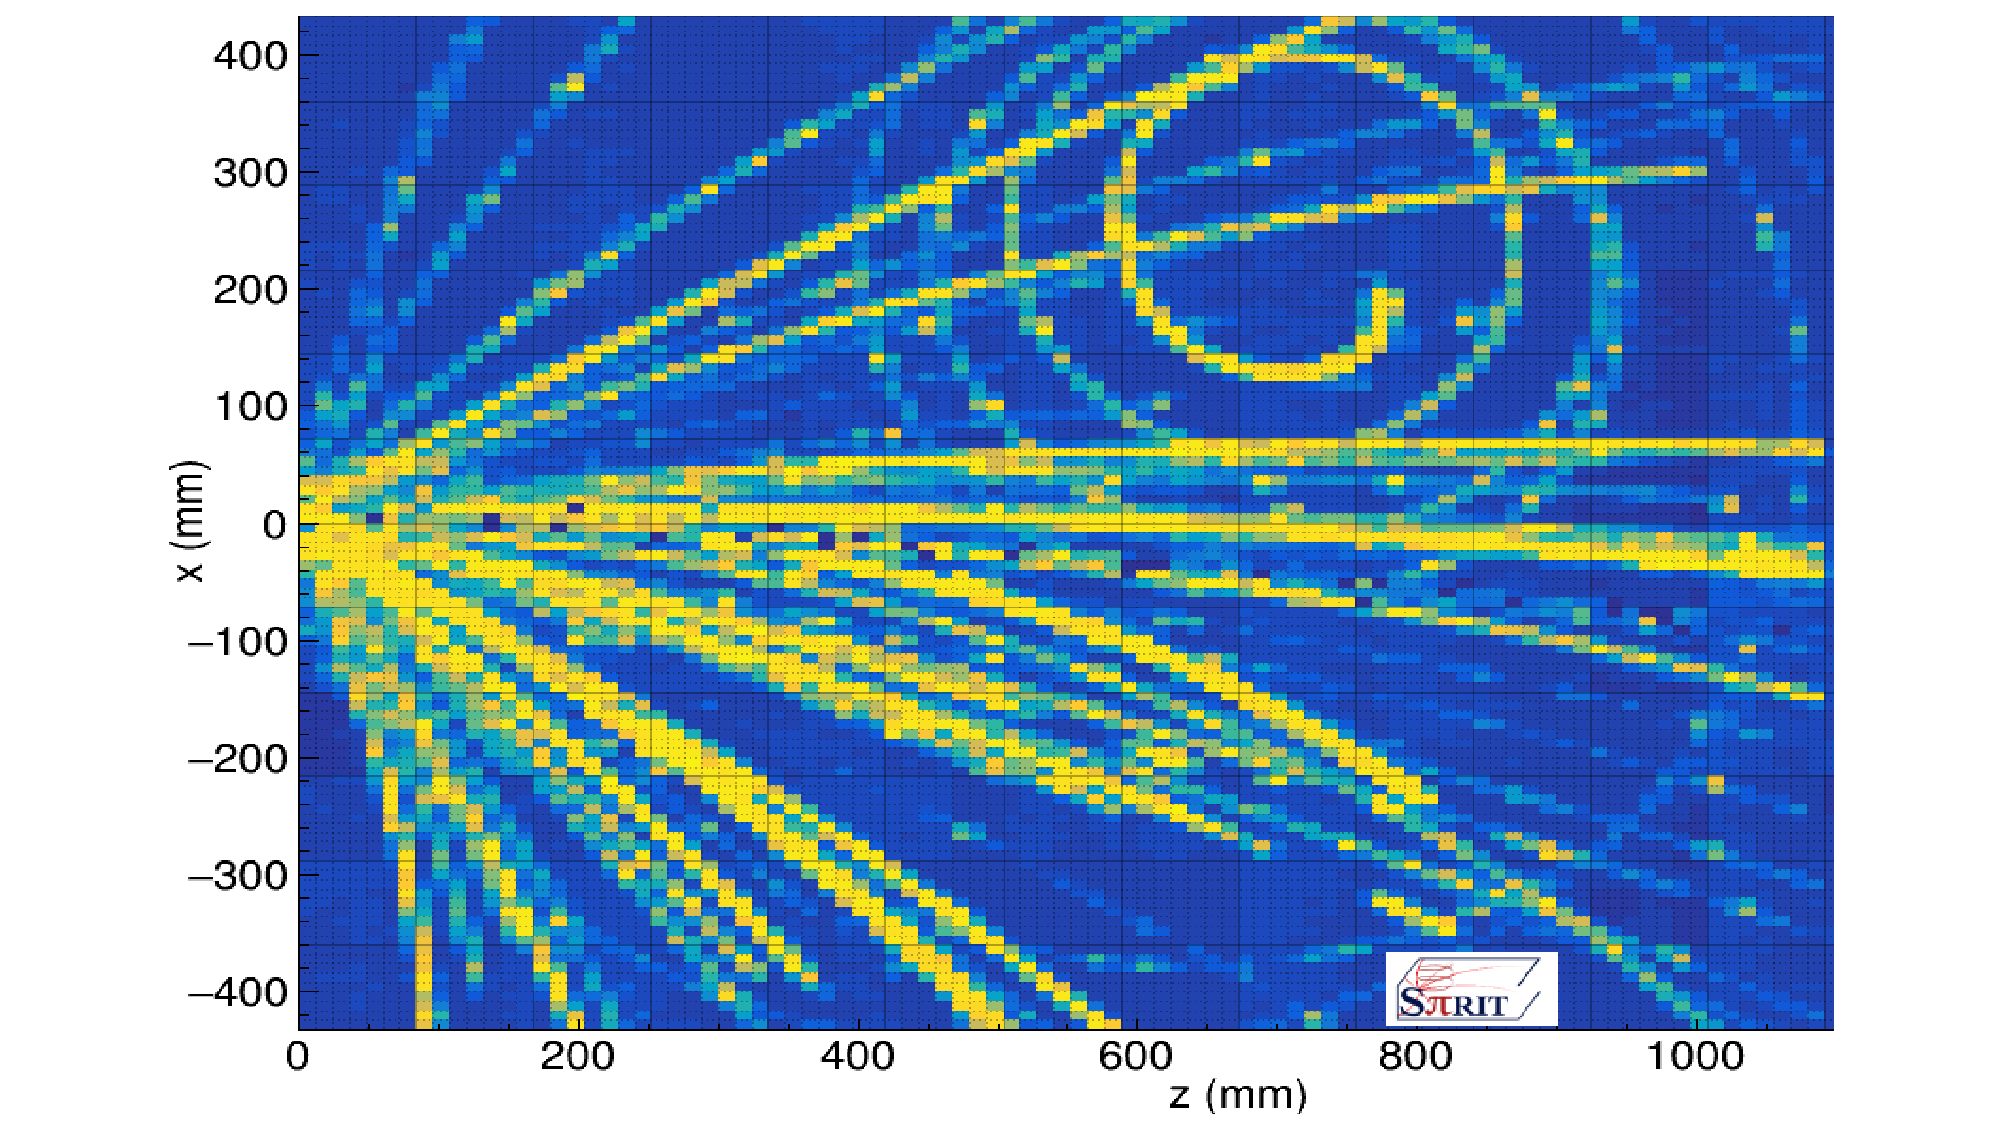
\includegraphics[width=0.45\linewidth]{figures/tracks_top_view.pdf}
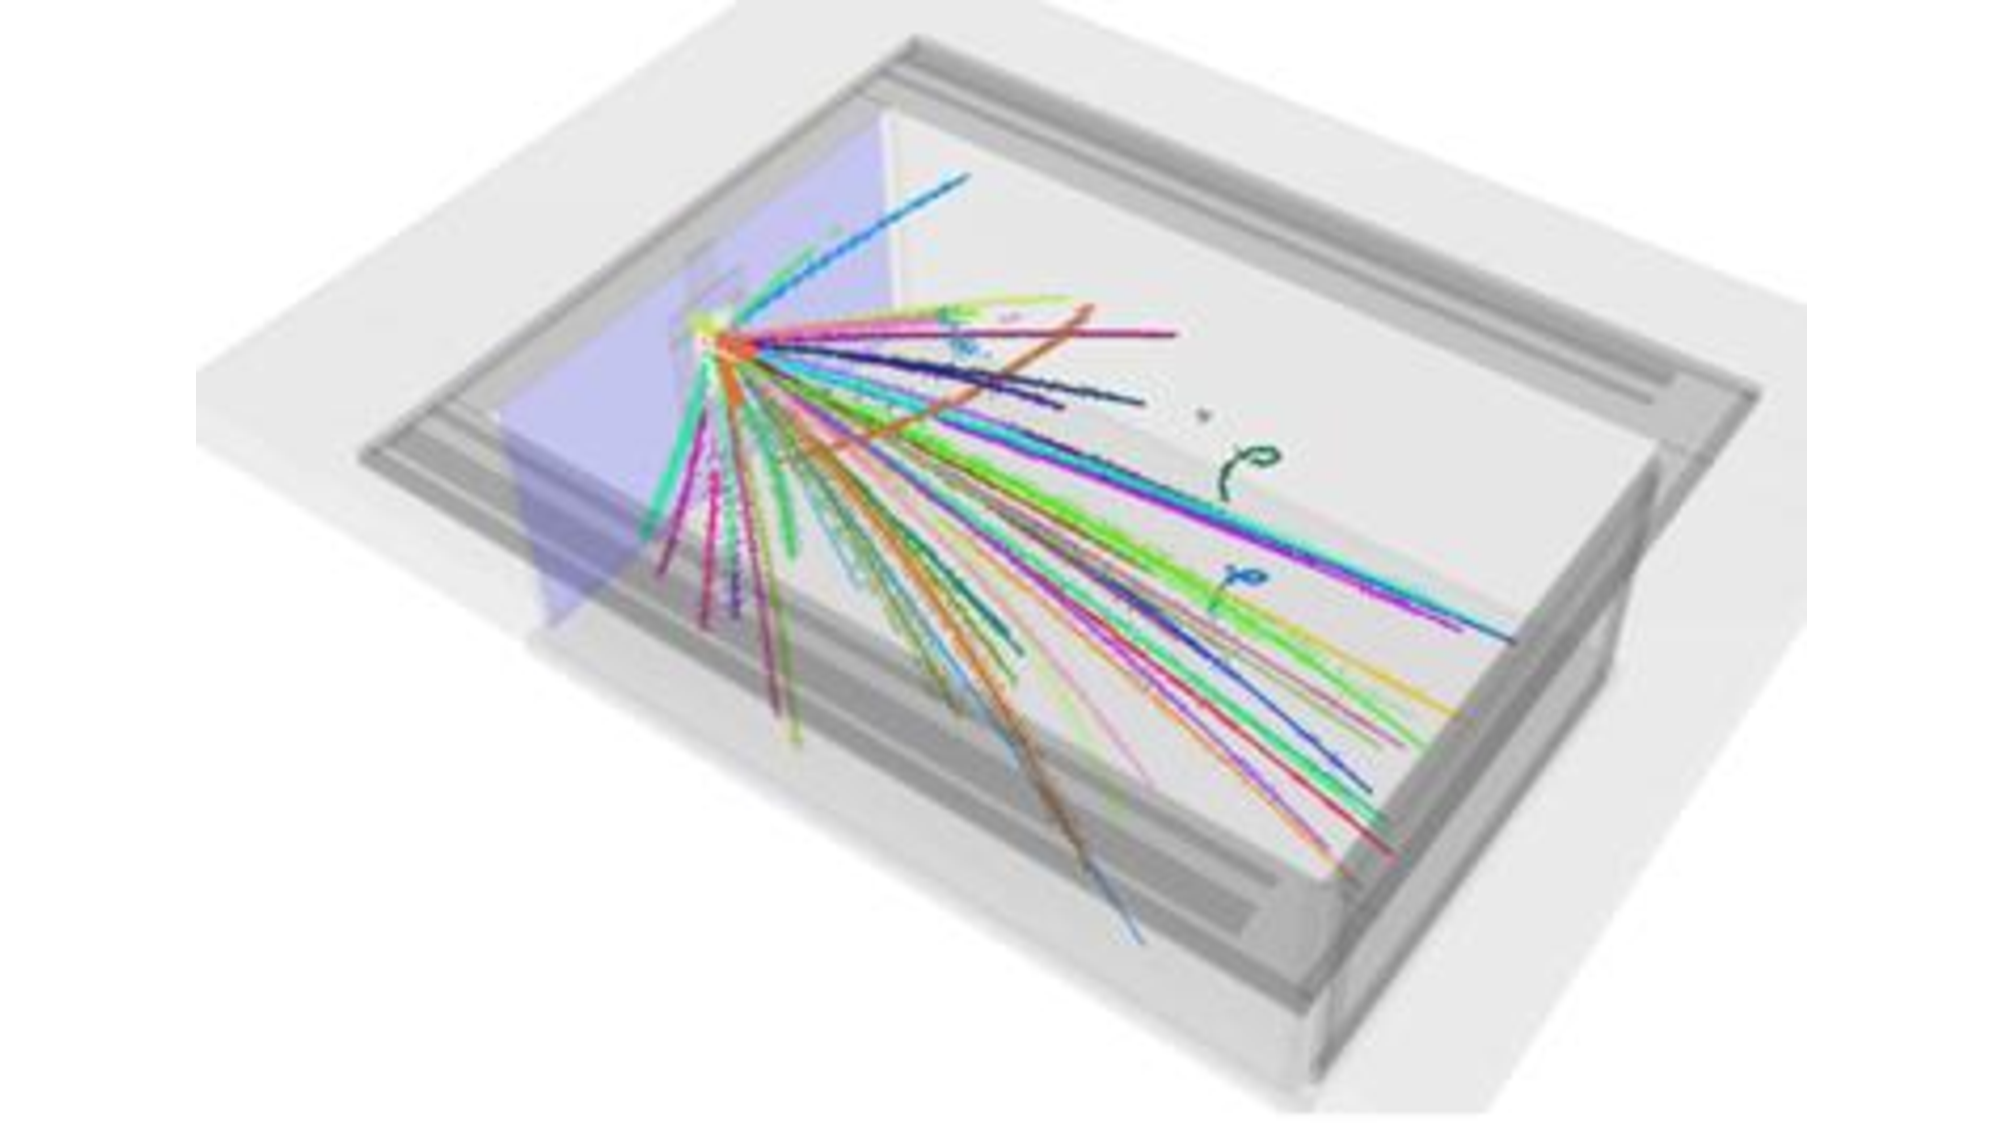
\includegraphics[width=0.45\linewidth]{figures/tracks_3d_view.pdf}
\caption{
Tracks from two different events from $^{132}Sn+^{124}Sn$ collisions as viewed from the top (left panel) and 3D (right panel). The big spiral in the left panel is an emitted low energy $\pi^-$.
}
\end{figure}
\clearpage
\newpage


\subsubsection{Pulse shape discrimination from digitized waveforms}

\vspace{5mm}

\noindent
\fbox{\begin{minipage}{0.98\linewidth}
\begin{description}
%%%
\item[Participants:] F.C.E. Teh (g), T. Ladourceur (u), C.Y. Tsang (g), M.B. Tsang
%%%
\item[Description:] With the advancement of digital electronics, we are able to record the waveforms of the signal pulses directly. That allows automation and innovation in data analysis. Depending on the detector materials, waveforms may contain information about the particle types and the corresponding energy. The figure below shows the waveforms identified using new improved method (right panel) to distinguish neutrons from gammas detected by a large array made from organic liquid scintillator from an experiment at NSCL. The pulse shape (left panel) depends on the position of the detector where the radiation hit. It is a complicated multi-correlation problem suitable for developing ML algorithm using separate data sets for training and validating.
%%%
\item[FRIB relevance:] Digital electronics  produces large amount of information and are increasingly used in nuclear physics experiments including those in FRIB. To exploit the full potential of digial electronics, fast ML algorithms must be developed to classify pulse shapes for different particle types in online or offline analysis.
%%%
\item[References:] {\it Value-assigned pulse shape discrimination for neutron detectors}, F.C.E. Teh, J.-W. Lee, K. Zhu, K.W. Brown, et al., \href{https://arxiv.org/abs/2001.07518}{arXiv:2001.07518}.
%%%
\end{description}
%%%
\end{minipage}
}

\begin{figure}[htb!]
\centering
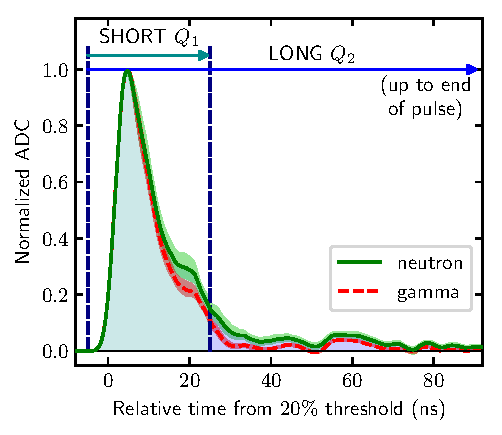
\includegraphics[width=0.49\linewidth]{figures/psd_median_pulse_shapes.pdf}
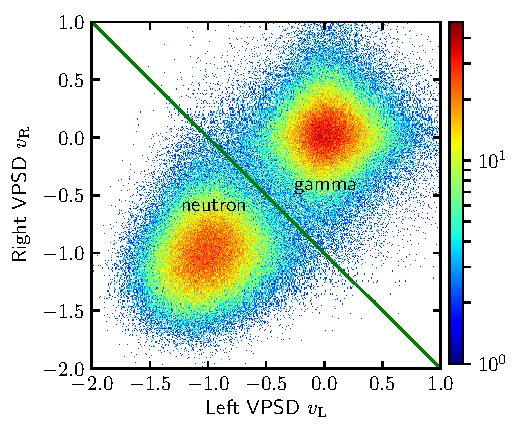
\includegraphics[width=0.49\linewidth]{figures/psd_2d_vpsd.pdf}
\caption{
(Left panel) Waveforms recorded by the Large Area Neutron Detector (LANA).  (Right panel) Valued-assigned pulse shape discrimination (VPSD) method developed to better discriminate neutrons and gamma.
}
\end{figure}
\clearpage
\newpage




\end{document}

